\input{"preamble.tex"}

\addbibresource{NumberTheory.bib}

\let\Begin\begin
\let\End\end
\newcommand\wrapenv[1]{#1}

\makeatletter
\def\ScaleWidthIfNeeded{%
 \ifdim\Gin@nat@width>\linewidth
    \linewidth
  \else
    \Gin@nat@width
  \fi
}
\def\ScaleHeightIfNeeded{%
  \ifdim\Gin@nat@height>0.9\textheight
    0.9\textheight
  \else
    \Gin@nat@width
  \fi
}
\makeatother

\setkeys{Gin}{width=\ScaleWidthIfNeeded,height=\ScaleHeightIfNeeded,keepaspectratio}%

\title{
\rule{\linewidth}{1pt} \\
\textbf{
    Algebraic Number Theory
  }
    \\ {\normalsize Lectures by Paul Pollack. University of Georgia,
Spring 2021} \\
  \rule{\linewidth}{2pt}
}
\titlehead{
    \begin{center}
  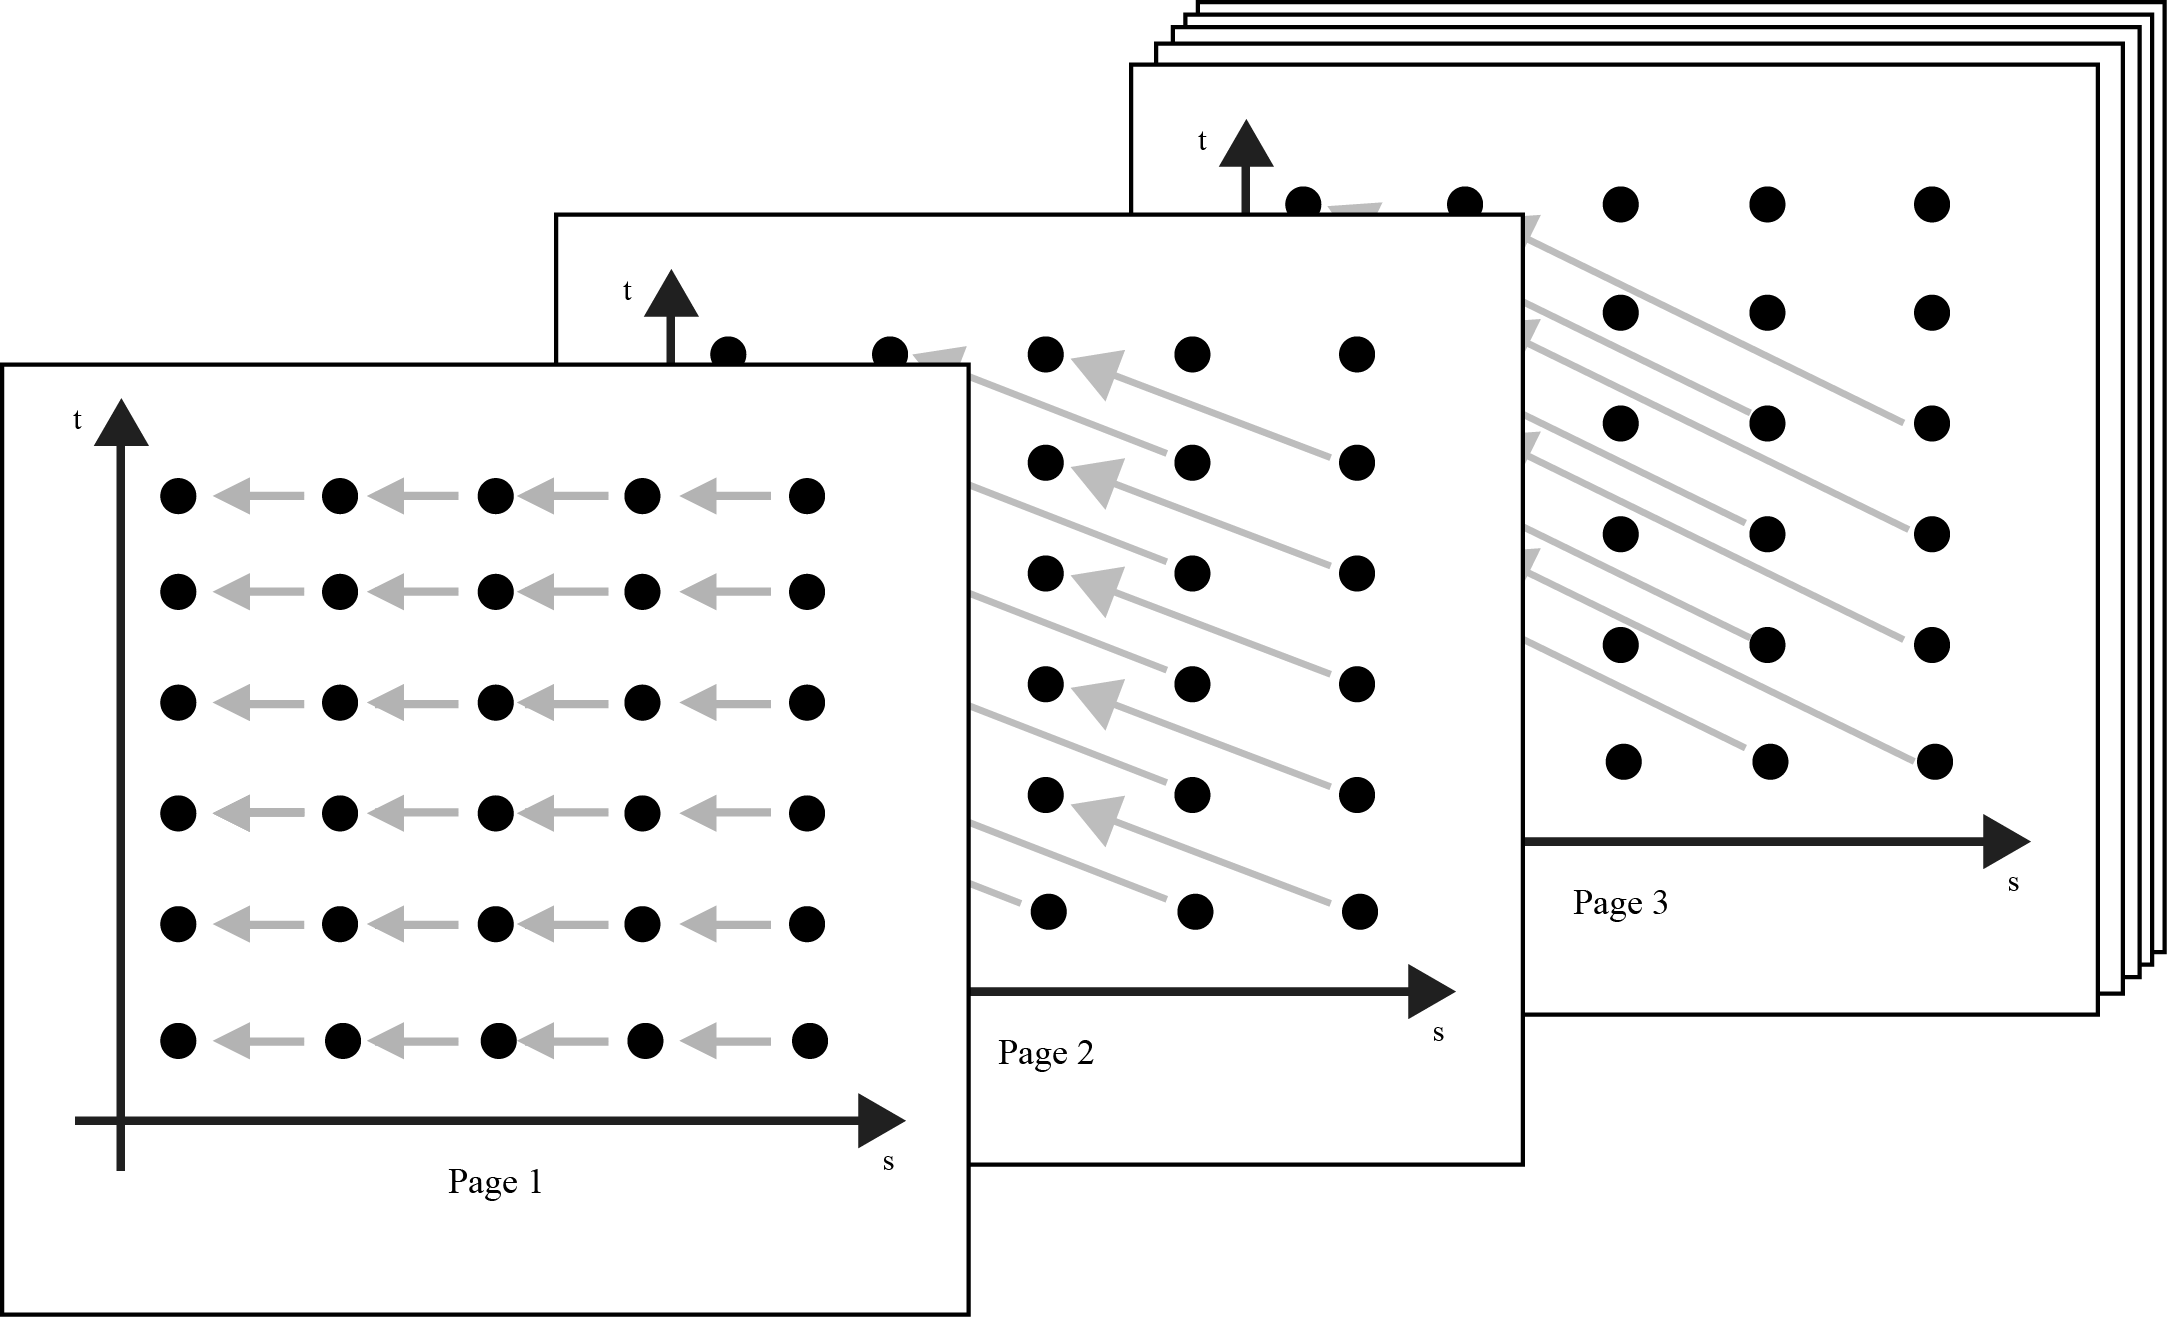
\includegraphics[width=\linewidth,height=0.45\textheight,keepaspectratio]{figures/cover.png}
  \end{center}
       \begin{minipage}{.35\linewidth}
    \begin{flushleft}
      \vspace{2em}
      {\fontsize{6pt}{2pt} \textit{Notes: These are notes live-tex'd
from a graduate course in Algebraic Number Theory taught by Paul Pollack
at the University of Georgia in Spring 2021. As such, any errors or
inaccuracies are almost certainly my own. } } \\
    \end{flushleft}
    \end{minipage}
    \hfill
    \begin{minipage}{.65\linewidth}
    \end{minipage}
  }







\begin{document}

\date{}
\author{D. Zack Garza}
\maketitle
\begin{flushleft}
\textit{D. Zack Garza} \\
\textit{University of Georgia} \\
  \textit{\href{mailto: dzackgarza@gmail.com}{dzackgarza@gmail.com}} \\
{\tiny \textit{Last updated:} 2021-01-28 }
\end{flushleft}


\newpage

% Note: addsec only in KomaScript
\addsec{Table of Contents}
\tableofcontents
\newpage

\def\contradiction
{
\tikz[baseline, x=0.2em, y=0.2em, line width=0.04em]
\draw (0,0) -- ({4*cos(45)},{4*sin(45)})
    (-1,1) -- ({-1 + 4*cos(45)},{1 + 4*sin(45)})
    (-1,3) -- ({-1 + 4*cos(315)},{3 + 4*sin(315)})
    (0,4) -- ({0 + 4*cos(315)},{4 + 4*sin(315)});
}

\hypertarget{thursday-january-14}{%
\section{Thursday, January 14}\label{thursday-january-14}}

See website for notes on books, intro to class.

\begin{itemize}
\item
  Youtube Playlist:
  \url{https://www.youtube.com/playlist?list=PLA0xtXqOUji8fjQysx4k8a6h-hOZ7x5ue}
\item
  Free copies of textbook:
  \url{https://www.dropbox.com/sh/rv5j222kn74bjhm/AABZ1qcR1rOnpaBsa5CL3P_Ea?dl=0\&lst=}
\item
  Course website: ?
\end{itemize}

Paul's description of the course:

``This course is an introduction to arithmetic''beyond
\({\mathbb{Z}}\)``, specifically arithmetic in the ring of''integers" in
a finite extension of \({\mathbb{Q}}\). (Among many other things) we'll
prove three important theorems about these rings:

\begin{itemize}
\tightlist
\item
  Unique factorization into ideals.
\item
  Finiteness of the group of ideal classes.
\item
  Dirichlet's theorem on the structure of the unit group."
\end{itemize}

\hypertarget{motivation}{%
\subsection{Motivation}\label{motivation}}

Solving Diophantine equations, i.e.~polynomial equations over
\({\mathbb{Z}}\).

\begin{example}[?]

Consider \(y^2 = x^3 + x\).

\begin{claim}

\((x, y) = (0, 0)\) is the only solution.

\end{claim}

To see this, write \(y^2 = x(x^2+1)\), which are relatively prime,
i.e.~no \(D\in {\mathbb{Z}}\) divides both of them. Why? If
\(d \divides x\) and \(d \divides x+1\), then
\(d\divides (x^2+1) + (-x) = 1\). It's also the case that both \(x^2+1\)
and \(x^2\) are squares (up to a unit), so \(x^2, x^2 + 1\) are
consecutive squares in \({\mathbb{Z}}\). But the gaps between squares
are increasing: \(1, 2, 4, 9, \cdots\). The only possibilities would be
\(x=0, y=1\), but in this case you can conclude \(y=0\).

\end{example}

\begin{example}[Fermat]

Consider \(y^2 = x^3-2\).

\begin{claim}

\((3, \pm 5)\) are the only solutions.

\end{claim}

Rewrite
\begin{align*}
x^3 = y^2+2 &= (y+ \sqrt{-2})(y - \sqrt{-2}) \\ 
&\in
{\mathbb{Z}}[\sqrt{-2}] \coloneqq\left\{{a+b\sqrt{-2} {~\mathrel{\Big|}~}a,b,\in {\mathbb{Z}}}\right\} \leq {\mathbb{C}}
.\end{align*}
This is a subring of \({\mathbb{C}}\), and thus at least an integral
domain. We want to try the same argument: showing the two factors are
relatively prime. A little theory will help here:

\begin{definition}[Norm Map]

For \(\alpha\in {\mathbb{Z}}[\sqrt{-2}]\) define
\(N \alpha = \alpha\mkern 1.5mu\overline{\mkern-1.5mu\alpha\mkern-1.5mu}\mkern 1.5mu\).

\end{definition}

\begin{lemma}[?]

Let \(\alpha, \beta \in {\mathbb{Z}}[\sqrt{-2}]\). Then

\begin{enumerate}
\def\labelenumi{\arabic{enumi}.}
\item
  \(N(\alpha \beta) = N(\alpha) N(\beta)\)
\item
  \(N( \alpha) \in {\mathbb{Z}}_{\geq 0}\) and \(N(\alpha) = 0\) if and
  only if \(\alpha= 0\).
\item
  \(N(\alpha) = 1 \iff \alpha\in R^{\times}\)
\end{enumerate}

\end{lemma}

\begin{proof}[?]

\begin{enumerate}
\def\labelenumi{\arabic{enumi}.}
\item
  Missing, see video (10:13 AM).
\item
  \(N(\alpha) = a^2 + 2b^2 \geq 0\), so this equals zero if and only if
  \(\alpha= \beta= 0\)
\item
  Write
  \(1 = \alpha\mkern 1.5mu\overline{\mkern-1.5mu\alpha\mkern-1.5mu}\mkern 1.5mu\)
  if \(N(\alpha) = 1 \in R^{\times}\). Conversely if
  \(\alpha\in R^{\times}\) write \(\alpha \beta = 1\), then
  \begin{align*} 
  1 = N(1) = N(\alpha \beta) = N(\alpha ) N(\beta ) \in {\mathbb{Z}}_{\geq 0} 
  ,\end{align*}
  which forces both to be 1.
\end{enumerate}

\end{proof}

\begin{claim}

The two factors \(y \pm \sqrt 2\) are \emph{coprime} in
\({\mathbb{Z}}[\sqrt{-2}]\), i.e.~every common divisor is a unit.

\end{claim}

\begin{proof}[?]

Suppose \(\delta\divides y\pm \sqrt{-2}\), then
\(y + \sqrt{-2} = \delta \beta\) for some
\(\beta\in {\mathbb{Z}}[\sqrt{-2}]\). Take norms to obtain
\(y^2 + 2 = N \delta N \beta\), and in particular

\begin{itemize}
\tightlist
\item
  \(N \delta y^2 +2\)
\item
  \(\delta \divides (y+ \sqrt{-2} ) - (y - \sqrt{-2} ) = 2 \sqrt{-2}\)
  and thus \(N \delta \divides N(2 \sqrt{-2} ) = 8\).
\end{itemize}

In the original equation \(y^2 = x^3-2\), if \(y\) is even then \(x\) is
even, and \(x^3 - 2 \equiv 0-2 \pmod 4 \equiv 2\), and so
\(y^2 \equiv 2 \pmod 4\). But this can't happen, so \(y\) is odd, and
we're done: we have \(N \delta\divides 8\) which is even or 1, but
\(N \delta\divides y^2 +2\) which is odd, so \(N \delta = 1\).

\end{proof}

We can identify the units in this ring:
\begin{align*}
{\mathbb{Z}}[\sqrt{-2} ]^{\times}= \left\{{ a + b \sqrt{-2} {~\mathrel{\Big|}~}a^2 + 2b^2 = 1}\right\}
\end{align*}
which forces \(a^2 \leq 1, b^2 \leq 1\) and thus this set is
\(\left\{{\pm 1}\right\}\).

So we have \(x^3 = ab\) which are relatively primes, so \(a,b\) should
also be cubes. We don't have to worry about units here, since \(\pm 1\)
are both cubes. So e.g.~we can write
\begin{align*}
y + \sqrt{-2} = (a + b \sqrt{-2} )^3 = (a^3-6ab^2) + (3a^2b -2b^3) \sqrt{-2}
.\end{align*}
Comparing coefficients of \(\sqrt{-2}\) yields
\begin{align*} 1 = b(3a^2b - 2b^2) \in {\mathbb{Z}}\implies b \divides 1
,\end{align*}
and thus \(b\in {\mathbb{Z}}^{\times}\),
i.e.~\(b\in \left\{{\pm 1}\right\}\). By cases:

\begin{itemize}
\item
  If \(b=1\), then \(1 = 3a^2 -2 \implies a^2 = 1 \implies a = \pm 1\).
  So
  \begin{align*}
  y = \sqrt{-2} = (\pm 1 + \sqrt{-2} )^3 = \pm 5 + \sqrt{-2}
  ,\end{align*}
  which forces \(y=\pm 5\), the solution we already knew.
\item
  If \(b = -1\), then \(1 = -(3a^2 - 1)\) which forces
  \(1=3a^2 \in {\mathbb{Z}}\), so there are no solutions.
\end{itemize}

\end{example}

\begin{example}[?]

Consider \(y^2 = x^3 - 26\). Rewrite this as
\begin{align*}
x^3 = y^2 + 26 = (y + \sqrt{-26} )(y - \sqrt{-26} )
,\end{align*}
then the same lemma goes through with \(2\) replaced by \(26\)
everywhere where the RHS factors are still coprime. Setting
\(y + \sqrt{-26} = (a + b \sqrt{-26} )^3\) and comparing coefficients,
you'll find \(b=1, a = \pm 3\). This yields \(x=35, y=\pm 207\). But
there are more solutions: \((x, y) = (3, \pm 1)\)! The issue is that we
used unique factorization when showing that \(ab\) is a square implies
\(a\) or \(b\) is a square (say by checking prime factorizations and
seeing even exponents). In this ring, we can have \(ab\) a cube with
\emph{neither} \(a,b\) a cube, even up to a unit.

\end{example}

\begin{question}

When does a ring admit unique factorization? Do you even \emph{need} it?

\end{question}

This will lead to a discussion of things like the \textbf{class number},
which measure the failure of unique factorization. In general, the above
type of proof will work when the class number is 3!

\hypertarget{lecture-2-tuesday-january-19}{%
\section{Lecture 2 (Tuesday, January
19)}\label{lecture-2-tuesday-january-19}}

Today: Ch.2 of the book, ``Cast of Characters''. Note that all rings
will be commutative and unital in this course.

Last time: looked at factorization in
\({\mathbb{Z}}[\sqrt 2], {\mathbb{Z}}[\sqrt{26}]\). Where do rings like
this come from?

\begin{definition}[Number Field]

A \textbf{number field} is a subfield \(K \subseteq {\mathbb{C}}\) such
that \([K: {\mathbb{Q}}] < \infty\).

\end{definition}

\begin{remark}

Some authors don't require \(K \subseteq {\mathbb{C}}\), but any finite
extension of \({\mathbb{Q}}\) will embed into \({\mathbb{C}}\) so
there's no harm in this extra requirement.

\end{remark}

\begin{example}[?]

\({\mathbb{Q}}[\sqrt[3]{2}, {\mathbb{Q}}[\sqrt 2, \sqrt[5]{7}]\) or
\({\mathbb{Q}}(\theta)\) where \(\theta\) is a root of \(x^5 - x - 1\)
(which you can check is irreducible. Now that the round vs.~square
brackets here won't make a difference, since we're adjoining algebraic
numbers.

\end{example}

\begin{proposition}[?]

Let \(K_{/{\mathbb{Q}}}\) be a finite extension, say of degree
\(n\coloneqq[K: {\mathbb{Q}}]\). Then there are \(n\) distinct
embeddings \footnote{An injective ring morphism.} of \(K\) into
\({\mathbb{C}}\)

\end{proposition}

\begin{proof}[?]

We have \(K_{/{\mathbb{Q}}}\), which is necessarily separable since
\(\operatorname{ch}({\mathbb{Q}}) = 0\). By the primitive element
theorem, we can write \(K = {\mathbb{Q}}(\theta)\) where \(\theta\) is a
root of some degree \(n\) irreducible polynomial
\(f(x) \in {\mathbb{Q}}[x]\). Since \({\mathbb{C}}\) is algebraically
closed, \(f\) splits completely over \({\mathbb{C}}\) as
\(f = \prod_{i=1}^n (x- \theta_i\) which each \(\theta_i \in CC\)
distinct since \(f\) was irreducible and we're in characteristic zero.
Then for each \(i\) there is an embedding \(K = {\mathbb{Q}}[\theta]\)
given by
\begin{align*}
\iota_i: {\mathbb{Q}}[\theta] &\hookrightarrow{\mathbb{C}}\\
g(\theta) &\mapsto g(\theta_i)
.\end{align*}
There are some easy things to check:

\begin{itemize}
\tightlist
\item
  This is well-defined: elements in \(K\) are polynomials in \(\theta\)
  but they all differ by a multiple of the minimal polynomial of
  \(\theta\),
\item
  This is an inject homomorphism and thus an embedding, and
\item
  For distinct \(i\) you get distinct embeddings: just look at the image
  \(\iota_i(\theta)\), these are distinct numbers in \({\mathbb{C}}\).
\end{itemize}

\end{proof}

\begin{definition}[Real and Nonreal embeddings]

Let \(K_{/{\mathbb{Q}}}\) be a finite extension of degree
\(n = [K : {\mathbb{Q}}]\). We'll say an embedding
\(\sigma:K \to {\mathbb{C}}\) is \textbf{real} if
\(\sigma(K) \subseteq {\mathbb{R}}\) , otherwise we'll say the embedding
is \textbf{nonreal}.

\end{definition}

\begin{remark}

If \(\sigma\) is a nonreal, then
\(\mkern 1.5mu\overline{\mkern-1.5mu\sigma\mkern-1.5mu}\mkern 1.5mu\) is
a nonreal embedding, so this embeddings come in pairs. As a consequence,
the total number of embeddings is given by \(n = r_1 + 2r_2\), where
\(r_1\) is the number of real embeddings and \(r_2\) is the number of
nonreal embeddings.

\end{remark}

\begin{example}[?]

Let \(K = {\mathbb{Q}}(\sqrt[3]{2})\). Here \(n=3\) since this is the
root of a degree 3 irreducible polynomial. Using the proof we can find
the embeddings: factor
\begin{align*}
x^3 - 2 = (x - \sqrt[3]{2})(x - \omega \sqrt[3]{2}) (x - \omega^2 \sqrt[3]{2})
.\end{align*}
where \(\omega = e^{2\pi i / 3}\) is a complex cube root of unity. We
can form an embedding by sending
\(\sqrt[3]{2} \to \omega^j \sqrt[3]{2}\) for \(j=0,1,2\). The case
\(j=0\) sends \(K\) to a subset of \({\mathbb{R}}\) and yields a real
embedding, but the other two will be nonreal. So \(r_1 = 1, r_2 = 1\),
and we have \(3 = 1 + 2(1)\) and this is consistent.

\end{example}

\begin{remark}

We've only been talking about fields, since unique factorization is
trivial since there are no primes. There are thus ``too many'' units,
compared to the rings we were considering before, so we'll restrict to
subrings. The question is: where is the arithmetic? Given a number field
\(K\), we want a ring \({\mathbb{Z}}_K\) that fits this analogy:

\begin{center}
\begin{tikzcd}
{\mathbb{Q}}\ar[dd] & \leadsto & K\ar[dd] \\
\\
{\mathbb{Z}}& \leadsto & {\mathbb{Z}}_K = ?
\end{tikzcd}
\end{center}

\end{remark}

\begin{definition}[Algebraic Numbers]

Given \(\alpha\in {\mathbb{C}}\) we say \(\alpha\) is an
\textbf{algebraic number} if and only if \(\alpha\) is algebraic over
\({\mathbb{Q}}\), i.e.~the root of some polynomial in
\({\mathbb{Q}}[x]\).

\end{definition}

\begin{remark}

We know that if we define
\(\mkern 1.5mu\overline{\mkern-1.5mu{\mathbb{Q}}\mkern-1.5mu}\mkern 1.5mu\coloneqq\left\{{\alpha\in {\mathbb{C}}{~\mathrel{\Big|}~}\alpha \text{ is algebraic over } {\mathbb{Q}}}\right\}\),
we can alternatively describe this as
\(\mkern 1.5mu\overline{\mkern-1.5mu{\mathbb{Q}}\mkern-1.5mu}\mkern 1.5mu= \left\{{ \alpha\in {\mathbb{C}}{~\mathrel{\Big|}~}[{\mathbb{Q}}(\alpha) : {\mathbb{Q}}] < \infty }\right\}\).
This is convenient because it's easy to see that algebraic numbers are
closed under sums and products, just using the ways degrees behave in
towers.

\end{remark}

\begin{corollary}[?]

\(\mkern 1.5mu\overline{\mkern-1.5mu{\mathbb{Q}}\mkern-1.5mu}\mkern 1.5mu\hookrightarrow{\mathbb{C}}\)
is a subfield and every number field is a subfield of
\(\mkern 1.5mu\overline{\mkern-1.5mu{\mathbb{Q}}\mkern-1.5mu}\mkern 1.5mu\).

\end{corollary}

These are still fields, so lets define some interesting subrings.

\begin{definition}[$\bar \ZZ$ ]

Define
\(\mkern 1.5mu\overline{\mkern-1.5mu{\mathbb{Z}}\mkern-1.5mu}\mkern 1.5mu\coloneqq\left\{{ \alpha\in {\mathbb{C}}{~\mathrel{\Big|}~}\alpha\text{ is the root of a monic polynomial }f\in {\mathbb{Z}}[x]}\right\}\).

\end{definition}

\begin{theorem}[$\bar \ZZ$ is a ring]

\(\mkern 1.5mu\overline{\mkern-1.5mu{\mathbb{Z}}\mkern-1.5mu}\mkern 1.5mu\)
is a ring, and in fact a domain since it's a subring of
\({\mathbb{C}}\).

\end{theorem}

We'll use an intermediate criterion to prove this:

\begin{proposition}[Integrality Criterion]

Let \(\alpha\in {\mathbb{C}}\) and suppose there is a finitely generated
\({\mathbb{Z}}{\hbox{-}}\)submodule of \({\mathbb{C}}\) with
\(\alpha M \subseteq M \neq 0\). Then
\(\alpha\in \mkern 1.5mu\overline{\mkern-1.5mu{\mathbb{Z}}\mkern-1.5mu}\mkern 1.5mu\),
i.e.~\(\alpha\) is the root of a monic polynomial with integer
coefficients.

\end{proposition}

\begin{proof}[of integrality criterion]

Chasing definitions, take \(M\) and choose a finite list of generators
\(\beta_1, \beta_2, \cdots, \beta_m\) for \(M\). Then
\(\alpha M \subseteq M \implies \alpha \beta_i \in M\) for all \(M\),
and each \(\alpha \beta_i\) is a \({\mathbb{Z}}{\hbox{-}}\)linear
combination of the \(\beta_i\) . I.e. we have
\begin{align*}
\alpha 
\begin{bmatrix}
\beta_1 
\\
\vdots  
\\
\beta_n  
\end{bmatrix}
= 
\begin{bmatrix}
a_{11} & a_{12} & \cdots
\\
a_{21} &  a_{22} & 
\\
 \vdots &  &\ddots  
\end{bmatrix}
\begin{bmatrix}
\beta_1 
\\
\vdots  
\\
\beta_n  
\end{bmatrix}
\coloneqq A \vec{\beta}
,\end{align*}
where \(A \in \operatorname{Mat}(n\times m, {\mathbb{Z}})\). We can
rearrange this to say that
\begin{align*}
\qty{ \alpha \operatorname{id}- A} 
\begin{bmatrix}
\beta_1 
\\
\vdots  
\\
\beta_n  
\end{bmatrix}
=
\mathbf{0}
.\end{align*}
Not all of the \(\beta_i\) can be zero since \(M\neq 0\), and thus
\(\alpha \operatorname{id}- A\) is singular and thus has determinant
zero, so \(\det(x \operatorname{id}- A)\Big|_{x=a} = 0\). We have
\begin{align*}
x\operatorname{id}- A = 
\begin{bmatrix}
x - a_{1,} &  & &
\\
&  x - a_{2, 2} & & 
\\
&  & \ddots &
\\
& &  & x - a_{m, m}
\end{bmatrix}
,\end{align*}
where the off-diagonal components are constants in \({\mathbb{Z}}\)
coming from \(A\). Taking the determinant yields a monic polynomial: the
term of leading degree comes from multiplying the diagonal components,
and expanding over the remaining minors only yields terms of smaller
degree. So \(\det (x\operatorname{id}- A) \in {\mathbb{Z}}[x]\) is
monic.

\end{proof}

\begin{proof}[of theorem]

We want to show that
\(\mkern 1.5mu\overline{\mkern-1.5mu{\mathbb{Z}}\mkern-1.5mu}\mkern 1.5mu\)
is a ring, and it's enough to show that

\begin{itemize}
\tightlist
\item
  \(1\in \mkern 1.5mu\overline{\mkern-1.5mu{\mathbb{Z}}\mkern-1.5mu}\mkern 1.5mu\),
  which is true since \(x-1\) is monic.
\item
  It's closed under \(+, \cdot\).
\end{itemize}

Note that the first property generalizes to
\({\mathbb{Z}}\subseteq \mkern 1.5mu\overline{\mkern-1.5mu{\mathbb{Z}}\mkern-1.5mu}\mkern 1.5mu\),
since \(x-n\) is monic for any \(n\in {\mathbb{Z}}\). For the second,
let
\(\alpha, \beta \in \mkern 1.5mu\overline{\mkern-1.5mu{\mathbb{Z}}\mkern-1.5mu}\mkern 1.5mu\).
Define \(M \coloneqq{\mathbb{Z}}[\alpha, \beta]\), then it's clear that
\((\alpha + \beta)M \subseteq M\) and \((\alpha \beta)M \subseteq M\)
since \({\mathbb{Z}}[\alpha, \beta]\) are polynomials in
\(\alpha, \beta\) and multiplying by these expression still yields such
polynomials. It only remains to check the following:

\begin{claim}

\(M\) is finitely-generated.

\end{claim}

\begin{proof}[?]

Let \(\alpha\) be a root of \(f \in {\mathbb{Z}}[x]\) and \(\beta\) a
root of \(g\), both monic with \(\deg f = n, \deg g = m\). We want to
produce a finite generating set for
\(M\coloneqq{\mathbb{Z}}[\alpha, \beta]\), and the claim is that the
following works:
\(\left\{{ \alpha^i \beta^j}\right\} _{\substack{0\leq i < n \\ 0 \leq j < m} }\),
i.e.~every element of \(M\) is some \({\mathbb{Z}}{\hbox{-}}\)linear
combination of these.

Note that this is clearly true if we were to include \(n, m\) in the
indices by collecting terms of any polynomial in \(\alpha, \beta\), so
the restrictions are nontrivial. It's enough to show that for any
\(0 \leq I, J \in {\mathbb{Z}}\), the term \(\alpha^I \beta^J\) is a
\({\mathbb{Z}}{\hbox{-}}\)linear combination of the restricted elements
above. Divide by \(f\) and \(g\) to obtain \(x^I = f(x) q(x) + r(x)\)
and \(x^J = g(x) \tilde q(x) \tilde r(x)\) where \(r(x) = 0\) or
\(\deg r < n\) and similarly for \(\tilde r\), where (importantly) all
of these polynomials are in \({\mathbb{Z}}[x]\).

We're not over a field: \({\mathbb{Z}}[x]\) doesn't necessarily have a
division algorithm, so why is this okay? The division algorithm only
requires inverting the leading coefficient, so in general \(R[x]\)
admits the usual division algorithm whenever the leading coefficient is
in \(R^{\times}\).

Now plug \(\alpha\) into the first equation to obtain
\(\alpha^I = r(\alpha)\) where \(\deg r < n\), which rewrite
\(\alpha^I\) as a sum of lower-degree terms. Similarly writing
\(\beta^J = r(\beta)\), we can express
\begin{align*}
\alpha^I \beta^J = r(\alpha) r(\beta)
,\end{align*}
which is what we wanted.

\end{proof}

\end{proof}

\begin{remark}

We've just filled in another part of the previous picture:

\begin{center}
\begin{tikzcd}
{\mathbb{Q}}\ar[dd] & K\ar[dd] & \mkern 1.5mu\overline{\mkern-1.5mu{\mathbb{Q}}\mkern-1.5mu}\mkern 1.5mu\ar[dd]\\
\\
{\mathbb{Z}}& {\mathbb{Z}}_K & \mkern 1.5mu\overline{\mkern-1.5mu{\mathbb{Z}}\mkern-1.5mu}\mkern 1.5mu
\end{tikzcd}
\end{center}

\end{remark}

\begin{definition}[Ring of Integers]

Define
\({\mathbb{Z}}_K = \mkern 1.5mu\overline{\mkern-1.5mu{\mathbb{Z}}\mkern-1.5mu}\mkern 1.5mu\cap K\),
the \textbf{ring of integers} of \(K\). Note that this makes sense since
the intersection of rings is again a ring.

\end{definition}

\begin{remark}

Why not just work in
\(\mkern 1.5mu\overline{\mkern-1.5mu{\mathbb{Z}}\mkern-1.5mu}\mkern 1.5mu\)?
It doesn't have the factorization properties we want, e.g.~there are no
irreducible elements. Consider \(\sqrt 2\), we can factor is into two
non-units (noting that \(\sqrt 2\) is not a unit) as
\(\sqrt{\sqrt 2} \cdot \sqrt{\sqrt 2}\), and it's easy to check that if
\(a\) is not a unit then \(\sqrt a\) is not a unit. So this would yield
arbitrarily long factorizations, and is thus not Noetherian.

\end{remark}

The following is a reality check, and certainly a property we would
want:

\begin{proposition}[The ring of integers of $\QQ$ is $\ZZ$ ]

\({\mathbb{Z}}_{\mathbb{Q}}= {\mathbb{Z}}\).

\end{proposition}

\begin{proof}[of proposition]

\(\subseteq\): easy, since
\({\mathbb{Z}}\subseteq \mkern 1.5mu\overline{\mkern-1.5mu{\mathbb{Z}}\mkern-1.5mu}\mkern 1.5mu\)
and \({\mathbb{Z}}\subseteq {\mathbb{Q}}\), and is thus in their
intersection \({\mathbb{Z}}_{\mathbb{Q}}\) .

\(\supseteq\) : Let
\(\alpha\in {\mathbb{Z}}_{\mathbb{Q}}= {\mathbb{Q}}\cap\mkern 1.5mu\overline{\mkern-1.5mu{\mathbb{Z}}\mkern-1.5mu}\mkern 1.5mu\)
, so \(\alpha\) is a root of
\(x^n - a_{n-1}x^{n-1} + \cdots + a_1x + a_0 \in {\mathbb{Z}}[x]\). We
know \(\alpha= a/b\) with \(a,b \in {\mathbb{Z}}\), and we can use the
rational root test which tells us that \(a\divides a_0, b\divides 1\),
so \(b = \pm 1, \alpha = a/\pm 1 = \pm a \in {\mathbb{Z}}\) and thus
\(\alpha \in {\mathbb{Z}}\).

\end{proof}

We'll want to study \({\mathbb{Z}}_K\) for various number fields \(K\),
but we'll need more groundwork.

\begin{proposition}[Easy criterion to check if an integer is algebraic]

Let
\(\alpha \in \mkern 1.5mu\overline{\mkern-1.5mu{\mathbb{Q}}\mkern-1.5mu}\mkern 1.5mu\),
then
\begin{align*} \alpha\in \mkern 1.5mu\overline{\mkern-1.5mu{\mathbb{Z}}\mkern-1.5mu}\mkern 1.5mu\iff \min_ \alpha \in {\mathbb{Z}}[x], \end{align*}
where \(\min_ \alpha(x)\) is the unique monic irreducible polynomial in
\({\mathbb{Q}}[x]\) which vanishes at \(\alpha\).

\end{proposition}

\begin{proof}[?]

\(\impliedby\): Trivial, if the minimal polynomial already has integer
coefficients, just note that it's already monic and thus
\(\alpha \in \mkern 1.5mu\overline{\mkern-1.5mu{\mathbb{Z}}\mkern-1.5mu}\mkern 1.5mu\)
by definition.

\(\implies\): Why should the minimal polynomial have \emph{integer}
coefficients? Choose a monic \(f(x) \in {\mathbb{Z}}[x]\) with
\(f(\alpha) = 0\), using the fact that
\(\alpha\in \mkern 1.5mu\overline{\mkern-1.5mu{\mathbb{Z}}\mkern-1.5mu}\mkern 1.5mu\)
, and factor \(f(x) = \prod_{i=1}^n (x- \alpha_i) \in {\mathbb{C}}[x]\).
Note that each
\(\alpha_i \in \mkern 1.5mu\overline{\mkern-1.5mu{\mathbb{Z}}\mkern-1.5mu}\mkern 1.5mu\)
since they are all roots of \(f\) (a monic polynomial in
\({\mathbb{Z}}[x]\)). Use the fact that \(\min_ \alpha(x)\) divides
every polynomial which vanishes on \(\alpha\) over \({\mathbb{Q}}\), and
thus divides \(f\) (noting that this still divides over
\({\mathbb{C}}\)). Moreover, every root of \(\min_ \alpha(x)\) is a root
of \(f\), and so every such root is some \(\alpha_i\).

Now factor \(\min_ \alpha(x)\) over \({\mathbb{C}}\) to obtain
\(\min_ \alpha(x) = \prod_{i=1}^m (x - \beta_i)\) with all of the
\(\beta_i \in \mkern 1.5mu\overline{\mkern-1.5mu{\mathbb{Z}}\mkern-1.5mu}\mkern 1.5mu\).
What coefficients appear after multiplying things out? Just sums and
products of the \(\beta_i\), so all of the coefficients are in
\(\mkern 1.5mu\overline{\mkern-1.5mu{\mathbb{Z}}\mkern-1.5mu}\mkern 1.5mu\)
. Thus
\(\min_ \alpha(x) \in \mkern 1.5mu\overline{\mkern-1.5mu{\mathbb{Z}}\mkern-1.5mu}\mkern 1.5mu[x]\).
But the coefficients are also in \({\mathbb{Q}}\) by definition, so the
coefficients are in
\(\mkern 1.5mu\overline{\mkern-1.5mu{\mathbb{Z}}\mkern-1.5mu}\mkern 1.5mu\cap{\mathbb{Q}}= {\mathbb{Z}}\)
and thus \(\min_ \alpha(x) \in {\mathbb{Z}}[x]\).

\end{proof}

\begin{example}[Showing an integer is not algebraic using minimal polynomials]

\(\sqrt{5}/ 3 \not\in \mkern 1.5mu\overline{\mkern-1.5mu{\mathbb{Z}}\mkern-1.5mu}\mkern 1.5mu\)
since \(\min_ \alpha(x) = x^2 - 5/9 \not\in {\mathbb{Z}}[x]\), so this
is not an algebraic integer.

\end{example}

\begin{proposition}[$\ff(\ZZ_K) = K$ ]

\envlist

\begin{enumerate}
\def\labelenumi{\alph{enumi}.}
\tightlist
\item
  \(\mkern 1.5mu\overline{\mkern-1.5mu{\mathbb{Z}}\mkern-1.5mu}\mkern 1.5mu\)
  has
  \(\mkern 1.5mu\overline{\mkern-1.5mu{\mathbb{Q}}\mkern-1.5mu}\mkern 1.5mu\)
  as its fraction field, and
\item
  For any number field \(K\), \({\mathbb{Z}}_K\) has \(K\) as its
  fraction field.
\end{enumerate}

Moreover, both of these statements follow from:

\begin{enumerate}
\def\labelenumi{\alph{enumi}.}
\setcounter{enumi}{2}
\tightlist
\item
  If
  \(\alpha\in \mkern 1.5mu\overline{\mkern-1.5mu{\mathbb{Q}}\mkern-1.5mu}\mkern 1.5mu\)
  then
  \(d \alpha\in \mkern 1.5mu\overline{\mkern-1.5mu{\mathbb{Z}}\mkern-1.5mu}\mkern 1.5mu\)
  for some \(d\in {\mathbb{Z}}^{\geq 0}\)
\end{enumerate}

\end{proposition}

\begin{remark}

Thus the subring is ``big'' in the sense that if you allow taking
quotients, you recover the entire field. That \(c\implies a,b\): suppose
you want to write
\(\alpha \in \mkern 1.5mu\overline{\mkern-1.5mu{\mathbb{Q}}\mkern-1.5mu}\mkern 1.5mu\)
as \(\alpha=p/q\) with
\(p,q \in \mkern 1.5mu\overline{\mkern-1.5mu{\mathbb{Z}}\mkern-1.5mu}\mkern 1.5mu\).
Use \(c\) to produce
\(d\alpha\in \mkern 1.5mu\overline{\mkern-1.5mu{\mathbb{Z}}\mkern-1.5mu}\mkern 1.5mu\),
then just take \(d\alpha /d\). The same argument works for \(b\).

\end{remark}

\begin{exercise}[?]

Prove the proposition!

\end{exercise}

\begin{proposition}[?]

Suppose
\(\alpha\in \mkern 1.5mu\overline{\mkern-1.5mu{\mathbb{C}}\mkern-1.5mu}\mkern 1.5mu\)
and \(\alpha\) is a root of a monic polynomial in
\(\mkern 1.5mu\overline{\mkern-1.5mu{\mathbb{Z}}\mkern-1.5mu}\mkern 1.5mu [x]\).
Then
\(\alpha\in \mkern 1.5mu\overline{\mkern-1.5mu{\mathbb{Z}}\mkern-1.5mu}\mkern 1.5mu\).

\end{proposition}

\begin{remark}

This says that if a number \(\alpha\) is the root of a monic polynomial
whose coefficients are \emph{algebraic} integers, then \(\alpha\) itself
is an algebraic integer coefficients. This corresponds to the fact that
integral over integral implies integral in commutative algebra.

\end{remark}

\begin{exercise}[Prove the proposition.]

Prove this! Can use the integrality criterion (slightly challenging),
can also use Galois theory.

\end{exercise}

\hypertarget{lecture-3-thursday-january-21}{%
\section{Lecture 3 (Thursday, January
21)}\label{lecture-3-thursday-january-21}}

Today: roughly corresponds to chapter 3 in the book. Goal: do all of the
big theorems in the setting of quadratic number fields, then redo
everything for general number fields.

\hypertarget{quadratic-number-fields}{%
\subsection{Quadratic Number Fields}\label{quadratic-number-fields}}

Simplest case: \({\mathbb{Q}}\), a degree 1 number field, so the next
simplest case is degree 2.

\begin{definition}[Quadratic Number Fields]

A field \(K\) is a \textbf{quadratic number field} if and only if \(K\)
is a number field and \([K: {\mathbb{Q}}] = 2\).

\end{definition}

\begin{remark}

Some notation: if \(d\in {\mathbb{R}}^{\times}\), then \(\sqrt d\) means
the \emph{positive} square root of \(d\) if \(d \geq 0\), and if \(d<0\)
this denotes \(i\sqrt{{\left\lvert {d} \right\rvert}}\).

\end{remark}

\begin{proposition}[?]

If \(K\) is a quadratic number field, then
\(K = {\mathbb{Q}}(\sqrt{d})\) for some squarefree \footnote{\emph{Squarefree}
  means not divisible by \(n^2\) for any \(n > 1\in {\mathbb{Z}}\), or
  equivalently not divisible by the square of any primes.}
\(d\in {\mathbb{Z}}\). Moreover, this \(d\) is uniquely determined by
\(K\), so all quadratic number fields are parameterized by the set of
squarefree integers.

\end{proposition}

\begin{proof}[?]

\textbf{Existence}: Since \([K: {\mathbb{Q}}] = 2\), we have
\(K\supsetneq {\mathbb{Q}}\) so pick
\(\alpha\in K\setminus{\mathbb{Q}}\) then \(K = {\mathbb{Q}}(\alpha)\).
Note that we could also furnish this \(\alpha\) from the primitive
element theorem, although this is overkill here. So \(\alpha\) is a root
of some degree 2 \(p\in {\mathbb{Q}}[x]\), and by scaling coefficients
we can replace this by \(p\in {\mathbb{Z}}[x]\). So write
\(p(x) = Ax^2 + Bx + C\), in which case we can always write
\(\alpha = {-B \pm \sqrt{B^2 - 4AC} \over 2A}\) where \(A\neq 0\) since
this would imply that \(\alpha\in{\mathbb{Q}}\). Writing
\(\Delta\coloneqq B^2 - 4AC\), we have
\(K = {\mathbb{Q}}(\alpha) = {\mathbb{Q}}(\sqrt{\Delta})\). This is
close to what we want -- it's \({\mathbb{Q}}\) adjoin some integer --
but we'd like it to be squarefree.

Now let \(f\in {\mathbb{Z}}^{\geq 0}\) be chosen such that
\(f^2 \divides \Delta\) and \(f\) is as large as possible, i.e.~the
largest square factor of \(\Delta\). Writing \(\Delta = f^2 - d\) where
\(d\) is whatever remains. Then \(d\) must be squarefree, otherwise if
\(d\) had a square factor bigger than 1, say \(d = r^2 d'\), in which
case \(f^2 r^2 > f^2\) would be a larger factor of \(\Delta\). So \(d\)
is squarefree, and \(\Delta = f \sqrt d\) and thus
\({\mathbb{Q}}(\Delta) = {\mathbb{Q}}(\sqrt{d})\).

\textbf{Uniqueness}: Well use some extra machinery.

\begin{definition}[Norm and Trace]

Let \(K\) be a number field with \(K_{/{\mathbb{Q}}}\) Galois. For each
\(\alpha\in K\) define
\begin{align*}
N(\alpha) &\coloneqq\prod_{\sigma\in \operatorname{Gal}(K_{/{\mathbb{Q}}})} \sigma(\alpha) && \text{the norm} \\
\operatorname{Tr}(\alpha) &\coloneqq\sum_{\sigma\in \operatorname{Gal}(K_{/{\mathbb{Q}}})} \sigma(\alpha) && \text{the trace}
.\end{align*}

\end{definition}

\begin{remark}

Why use these kind of sum at all? Applying any element in the Galois
group just permutes the elements. Note that
\(N( \alpha), \operatorname{Tr}( \alpha)\) are
\(G(K_{/{\mathbb{Q}}}){\hbox{-}}\)invariant, and thus rational numbers
in \({\mathbb{Q}}\). The norm is multiplicative, and the trace is
additive and in fact \({\mathbb{Q}}{\hbox{-}}\)linear:
\(\operatorname{Tr}(a \alpha + b \beta) = a \operatorname{Tr}( \alpha) + b \operatorname{Tr}( \beta)\)
for all \(\alpha, \beta\in K\) and all \(a,b \in {\mathbb{Q}}\).

\end{remark}

What do the norm and trace look like for a quadratic field? We can write
\(K = \left\{{a + b \sqrt d {~\mathrel{\Big|}~}a,b \in {\mathbb{Q}}}\right\}\)
and there is a unique (non-identity) element
\(g\in \operatorname{Gal}(K_{/{\mathbb{Q}}})\) with
\(\sigma(a + b \sqrt d = a - b \sqrt{d}\). We'll refer to this
automorphism as \textbf{conjugation}. We can compute
\begin{align*}
N(a + b \sqrt{d} ) &= a^2 - db^2 \\
\operatorname{Tr}(a + b \sqrt{d} ) &= 2a
.\end{align*}

Returning to the proof, suppose otherwise that
\(K = {\mathbb{Q}}(\sqrt{d_1} ) = {\mathbb{Q}}( \sqrt{d_2} )\) with
\(d_1\neq d_2\) squarefree integers. Note that they must have the same
sign, otherwise one of these extensions would not be a subfield of
\({\mathbb{R}}\). We know \(\sqrt{d_1} \in {\mathbb{Q}}( \sqrt{d_2} )\)
and thus \(\sqrt{d_1} = a + b \sqrt{d_2}\) for some
\(a, b\in {\mathbb{Q}}\). Taking the trace of both sides, the LHS is
zero and the RHS is \(2a\) and we get \(a=0\) and
\(\sqrt{d_1} = b \sqrt{d_2}\). Write \(b = u/v\) with
\(u,v\in {\mathbb{Q}}\). Squaring both sides yields
\(v^2 d_1 = u^2 d_2\). Let \(p\) be a prime dividing \(d_1\); then since
\(d_1\) is squarefree there is only one copy of \(p\) occurring in its
factorization. Moreover there are an even number of copies of \(p\)
coming from \(v^2\), thus forcing \(d_2\) to have an odd power of \(p\).
This forces \(p\divides d_2\), and since this holds for every prime
factor \(p\) of \(d_1\), we get \(d_1 \divides d_2\) since \(d_1\) is
squarefree. The same argument shows that \(d_2 \divides d_1\), so
they're the same up to sign: but the signs must match and we get
\(d_1 = d_2\).

\end{proof}

Note that this results holds for every squarefree number not equal to 1.

\begin{question}

If \(K = {\mathbb{Q}}( \sqrt{d} )\), what is the ring of integers
\({\mathbb{Z}}_K\)? Some more machinery will help here.

\end{question}

\begin{definition}[The Field Polynomial of an Element]

Assume \(K_{/{\mathbb{Q}}}\) is a Galois number field and for
\(\alpha\in K\) define
\begin{align*}
\varphi_{\alpha}(x) \coloneqq\prod_{ \sigma\in \operatorname{Gal}(K_{/{\mathbb{Q}}})} \qty{ x - \sigma(\alpha)}
.\end{align*}

\end{definition}

\begin{remark}

For the same reasons mentioned for the norm/trace, we get
\(\varphi_{\alpha} \in {\mathbb{Q}}[x]\), and moreover
\(\varphi_{ \alpha } (\alpha) = 0\).

\end{remark}

When is \(\alpha\in {\mathbb{Z}}_K\)? We have the following criterion:

\begin{proposition}[?]

\begin{align*}
\alpha\in {\mathbb{Z}}_K \iff \varphi_{ \alpha } (x) \in {\mathbb{Z}}[x]
.\end{align*}

\end{proposition}

\begin{proof}[?]

\(\impliedby\): This is easy, since if \(\varphi_\alpha\) is a monic
polynomial with integer coefficients, meaning that \(\alpha\) is an
algebraic integer and thus in \({\mathbb{Z}}_K\).

\(\implies\): If \(\alpha \in {\mathbb{Z}}_K\) then it's the root of
some monic polynomial in \({\mathbb{Z}}[x]\), and the same is true for
\(\sigma(\alpha)\) and thus each
\(\sigma(\alpha) \in \mkern 1.5mu\overline{\mkern-1.5mu{\mathbb{Z}}\mkern-1.5mu}\mkern 1.5mu\).
So
\(\varphi_{ \alpha}(x) \in \mkern 1.5mu\overline{\mkern-1.5mu{\mathbb{Z}}\mkern-1.5mu}\mkern 1.5mu[x]\).
We said \(\varphi_{ \alpha}\) has coefficients in \({\mathbb{Q}}\) too,
and thus in
\(\mkern 1.5mu\overline{\mkern-1.5mu{\mathbb{Z}}\mkern-1.5mu}\mkern 1.5mu\cap{\mathbb{Q}}= {\mathbb{Z}}\).
So the problem is reduced to finding out when \(\varphi_{\alpha}(x)\)
has integer coefficients.

If \(\deg(K_{/{\mathbb{Q}}}) = n\), then
\begin{align*}
\varphi_{ \alpha}( \alpha) = \prod x- \sigma(\alpha) = x^n - \operatorname{Tr}(\alpha)x^{n-1} + \cdots + (-1)^n N( \alpha)
.\end{align*}
If \(n=2\), these are the only terms, and so if \(K\) is a quadratic
number field then \(\alpha\in K\) is in \({\mathbb{Z}}_K\) if and only
if \(\operatorname{Tr}( \alpha), N(\alpha) \in {\mathbb{Z}}\).

\end{proof}

\begin{example}[?]

Let \(K = {\mathbb{Q}}( \sqrt{5} )\), then is it true that
\({\mathbb{Z}}_K = {\mathbb{Z}}[\sqrt{5} ]\)? Since
\(1, \sqrt{5} \in {\mathbb{Z}}_K\), we have \(\supseteq\) since
\(1, \sqrt{5}\) are algebraic. The answer is \textbf{no}: take
\(\alpha\coloneqq{1 + \sqrt{5} \over 2}\), then \(N( \alpha) -4/4 = -1\)
and \(\operatorname{Tr}( \alpha) = 1\). These are integers, so
\(\alpha\in {\mathbb{Z}}_K\), and in fact \(\alpha\) is a root of
\(x^2 - x - 1 \in {\mathbb{Z}}[x]\).

\end{example}

\begin{theorem}[?]

Let \(K = {\mathbb{Q}}( \sqrt{d} )\) be a quadratic number field. Then
if \(d = 2,3 \pmod 4\), then
\({\mathbb{Z}}_K = \left\{{ a + b \sqrt{d} {~\mathrel{\Big|}~}a, b\in {\mathbb{Z}}}\right\}\).
If \(d=1 \pmod 4\), then
\({\mathbb{Z}}_K = \left\{{ {1 + b \sqrt{d} \over 2} {~\mathrel{\Big|}~}a,b\in {\mathbb{Z}},\, a\equiv b \pmod 2}\right\}\).

\end{theorem}

\begin{remark}

For \(d=1\), if \(a, b\) are even then we just recover the \(d=2,3\)
case, so we're picking up extra elements from when \(a,b\) both odd.

\end{remark}

\begin{proof}[?]

Let \(\alpha\in K\) and write \(\alpha = A + B \sqrt{d}\) with
\(A, B\in {\mathbb{Q}}\).

\begin{exercise}[?]

Check that \(N( \alpha), \operatorname{Tr}( \alpha) \in {\mathbb{Z}}\)
for both cases.

\end{exercise}

Assuming now that
\(N( \alpha), \operatorname{Tr}( \alpha) \in {\mathbb{Z}}\), then
\(A^2 - dB^2 \in {\mathbb{Z}}\). Multiply this by 2 to get
\((2A)^2 - d(2B)^2 \in 4{\mathbb{Z}}\). Recalling that
\(\operatorname{Tr}( \alpha) = 2 A\), we have
\((2A)^2 \in {\mathbb{Z}}\) and thus \(d(2B)^2 \in {\mathbb{Z}}\) as
well. The claim now is that \(2B \in {\mathbb{Z}}\): we know
\(2B\in {\mathbb{Q}}\). If \(2B\not\in {\mathbb{Z}}\), then the
denominator has some prime factor. This prime factor appears twice in
\((2B)^2\), and \(d(2B)^2 \in {\mathbb{Z}}\) then means that two copies
of \(p\) appear in \(d\) in order to cancel -- however, we assumed \(d\)
was squarefree. We now know that \(A, B \in {1\over 2}{\mathbb{Z}}\), so
write \(A = (1/2)a'\) and \(B = (1/2)b'\). Writing
\(\alpha= (1/2)a' + (1/2)b' \sqrt{d}\), we find that
\(N( \alpha) = ((a')^2 - d(b')^2) / 4 \in {\mathbb{Z}}\). So the
numerator is a multiple of 4, which yields
\((a')^2 \equiv d(b')^2 \pmod 4\). We proceed by cases.

\textbf{Case 1:} \(d = 2,3 \pmod 4\). If \(b'\) is odd then
\((b')^2 = 1\pmod 4\), which holds for any odd number. But then
\((a')^2 = d(b')^2 = d \pmod 4\), which is a problem -- squares modulo 4
can only be \(0\) or \(1\). This is a contradiction, so \(b'\) must be
even. Then \((b')^2 \pmod 4 = 0\), which forces \(a' \equiv 0 \pmod 4\)
and \(a'\) must be even. But if \(a', b'\) are both even,
\((1/2)a', (1/2)b'\in {\mathbb{Z}}\) and we obtain
\(\alpha\in {\mathbb{Z}}+ \sqrt{d} {\mathbb{Z}}\) .

\textbf{Case 2:} If \(d\equiv 1 \pmod 4\), then
\((a')^2 \equiv (b')^2 \pmod 4\). We can conclude that \(a', b'\) are
either both odd or both even, otherwise we'd get \(0\equiv 1 \pmod 4\),
and thus we can write \(a' \equiv b' \pmod 2\). But this was exactly the
condition appearing in the theorem.

\end{proof}

\begin{remark}

Let \(K\) be a quadratic number field. Then we can reformulate the
previous results as:

\begin{align*}
{\mathbb{Z}}_K = 
\begin{cases}
{\mathbb{Z}}[ \sqrt{d} ] &  d \equiv 2,3 \pmod 4
\\
{\mathbb{Z}}\left[{1 + \sqrt{d} \over 2}\right] & d \equiv 1 \pmod 4.
\end{cases}
\end{align*}

We've also shown that \({\mathbb{Z}}_K\) is a free
\({\mathbb{Z}}{\hbox{-}}\)module of rank 2, with basis either
\(\left\{{ 1, \sqrt{d} }\right\}\) or
\(\left\{{ 1, {1 + \sqrt{d} \over 2 } }\right\}\).

\end{remark}

\begin{remark}

What is true for general number fields? Important theorem:
\({\mathbb{Z}}_K\) is always a free \({\mathbb{Z}}{\hbox{-}}\)module,
i.e.~there always exists an \emph{integral basis}. Surprisingly, the
it's not always true that \({\mathbb{Z}}_K = {\mathbb{Z}}[\ell]\) for
\(\ell\) a single element.

\end{remark}

\hypertarget{lecture-4-wednesday-january-27}{%
\section{Lecture 4 (Wednesday, January
27)}\label{lecture-4-wednesday-january-27}}

Today: the failure of unique factorization. Roughly corresponds to
chapter 4: ``Paradise Lost''!

Setup: \(K\) is a quadratic field, a degree 2 extension of
\({\mathbb{Q}}\), which can be written as \(K = {\mathbb{Q}}(\sqrt{d})\)
with \(d\) squarefree. Last time, we completely described
\({\mathbb{Z}}_K\) (the algebraic integers in \(K\)):
\begin{align*}
{\mathbb{Z}}_K = 
\begin{cases}
{\mathbb{Z}}[ \sqrt{d} ] &  d \equiv 2,3 \pmod 4
\\
{\mathbb{Z}}\left[{1 + \sqrt{d} \over 2}\right] & d \equiv 1 \pmod 4.
\end{cases}
\end{align*}
We saw that the second admitted a different description as
\(\left\{{ {a + b \sqrt{d} \over 2}}\right\}\) where \(a,b\) are either
both even or both odd. Note that we can do interesting arithmetic in
\({\mathbb{Z}}_K\), but it's not necessarily well-behaved:
\({\mathbb{Z}}_K\) is not always a UFD. Letting \(d=-5\), we have
\({\mathbb{Z}}_K = {\mathbb{Z}}[ \sqrt{-5} ]\) where \(6\) factors in
two ways: \(6 = (1 + \sqrt{5} )(1 - \sqrt{-5} ) = (2)(3) = 6\).

Note that this isn't quite enough to show failure of unique
factorization, e.g.~we can factor \(16 = (4)(4) = (2)(8)\). Here you
should check that all 4 factors are irreducible, and that the factors on
the right aren't unit multiples of the ones on the left. For example,
\(21 = (-7)(-3) = (7)(3)\), but the factors only differ by the unit
\(-1\in {\mathbb{Z}}^{\times}\). The key to checking all of those: the
\textbf{norm map}:
\begin{align*}
N(a + b \sqrt{-5} ) = (a + b \sqrt{-5} ) (a - \sqrt{-5} ) = a^2 + 5b^2
.\end{align*}
where the second factor was the \emph{conjugate}, i.e.~the image of the
element under the nontrivial element of the Galois group of
\(K_{/{\mathbb{Q}}}\). If \(a + b \sqrt{-5} \in {\mathbb{Z}}_K\), then
\(N(a + b \sqrt{-5} \in {\mathbb{Z}}_{\geq 0}\) and is equal to zero if
and only if \(a + b \sqrt{-5} = 0\). Moreover, this is a unit if and
only if its norm is 1, \footnote{\(\impliedby\): If the norm is 1, the
  conjugate is the inverse. For the reverse direction, the argument was
  more complicated, and reduced to showing norms of units are \(\pm 1\),
  and positivity forces it to be \(1\).} i.e.~\(a^2 + 5b^2 = 1\), which
forces \(b=0\) and \(a=\pm 1\). So
\(U({\mathbb{Z}}[ \sqrt{-5} ] ) = \left\{{\pm 1}\right\}\).

We'll show one of the factors is irreducible, \(1 + \sqrt{-5}\). Recall
that \(x\in R\) a domain is \emph{irreducible} if and only if whenever
\(x = ab\), one of \(a,b\) is a unit. It itself is not a unit, since
\(N(1 + \sqrt{-5 }) = 6 \neq 1\). So suppose
\(1 + \sqrt{-5} = \alpha \beta\). Then
\begin{align*}
6 = N(\alpha \beta ) = N( \alpha) N( \beta)
,\end{align*}
and so up to reordering, we have \(N \alpha = 2, N \beta= 3\). Writing
\(\alpha= a + b \sqrt{-5}\) and taking norms yields \(2 = a^2 + 5b^2\),
which has no solutions: considering the equation \(\pmod 5\) yields
\(2\equiv a^2\), but \(2\) is not a square in
\({\mathbb{Z}}/5{\mathbb{Z}}\). \(\contradiction\)

Note that the only other way of factoring \(6\) is \(6=(1)(6)\), and
taking norms shows that one factor is a unit. So if we assume
\(\alpha, \beta\) aren't units, both \(N \alpha, N \beta > 1\), which
leads to the previous situation. By similar arguments, all 4 factors are
irreducible.

To see that the LHS factors aren't unit multiples of the RHS factors, we
can use the fact that the units are \(\pm 1\), and multiplying the LHS
by \(\pm 1\) can't yield \(2\) or \(3\). So this is a genuine
counterexample to unique factorization.

\hypertarget{factorization-theory}{%
\subsection{Factorization Theory}\label{factorization-theory}}

What went wrong in the previous example? We'll use a big of terminology
from an area of algebra called \emph{factorization theory}. Many
concepts related to divisibility can be discussed in this language!

\begin{definition}[Monoid]

A \textbf{monoid} is a nonempty set with a commutative associative
binary operation \(\cdot\) with an identity \(1\). We say a monoid is
\textbf{cancellative} if and only if whenever
\(\alpha \beta= \beta \alpha\) or \(\beta \alpha = \gamma \alpha\) then
\(\beta = \gamma\).

\end{definition}

\begin{definition}[Terminology for Cancellative Monoids]

A bunch of definitions: let \(M\) be a cancellative monoid.

\begin{itemize}
\tightlist
\item
  \(\alpha\divides \beta\) if and only if \(\beta= \alpha \gamma\) for
  some \(\gamma\).
\item
  \(\epsilon\) is a \textbf{unit} if \(\epsilon\divides 1\).
\item
  \(\alpha , \beta\) are \textbf{associates} if
  \(\alpha = \epsilon \beta\) for some unit \(\epsilon\)
\item
  \(\pi\in M\) is \textbf{irreducible} if and only if \(\pi\) is a unit
  and whenever \(\pi= \alpha \beta\) then either \(\alpha\) or \(\beta\)
  is a unit.
\item
  \(\pi \in M\) is \textbf{prime} whenever \(\pi\divides \alpha \beta\)
  then \(\pi\divides \alpha\) or \(\pi\divides \beta\).
\item
  \(\delta \in M\) is a greatest common divisor of \(\alpha, \beta\) if
  and only if \(\delta\) is a common divisor that is divisible by every
  other common divisor.
\item
  \(M\) is a \textbf{unique factorization monoid} if and only if every
  nonunit element in \(M\) factors uniquely as a product of irreducibles
  (uniqueness up to order and associates).
\end{itemize}

\end{definition}

\begin{remark}

Given \(R\) an integral domain, then \(R\setminus\left\{{0}\right\}\)
with multiplication is a cancellative monoid. Moreover,
\(R\setminus\left\{{0}\right\}\) is a unique factorization monoid if and
only if \(R\) is a UFD.

\end{remark}

\begin{question}

How do you show something is a UFD?

\end{question}

How does this proof go for \({\mathbb{Z}}\)?

\begin{itemize}
\tightlist
\item
  Use existence of a division algorithm
\item
  Prove Euclid's lemma: every irreducible is prime
\item
  Use factorization into irreducibles and proceed by induction (writing
  out two factorizations and cancelling things out in a combinatorial
  way)
\end{itemize}

So we'd like

\begin{enumerate}
\def\labelenumi{\arabic{enumi}.}
\tightlist
\item
  To know that irreducibles are prime, and
\item
  Everything to factor into irreducibles.
\end{enumerate}

\begin{definition}[Atomic]

For \(M\) a cancellative monoid, \(M\) is \textbf{atomic} if every
nonunit element of \(M\) is a product of irreducibles.

\end{definition}

\begin{proposition}[?]

Let \(M\) be a cancellative monoid, then \(M\) is a UFM if and only if
\(M\) is atomic and every irreducible is prime in \(M\).

\end{proposition}

\begin{proof}[?]

Omitted -- no new ideas when compared to proof of unique factorization
in \({\mathbb{Z}}\).

\end{proof}

Note that in \({\mathbb{Z}}\), working in \({\mathbb{Z}}_{\geq 0}\) is
useful because the only positive unit is \(1\), and so any elements
differing by a unit are in fact equal. Can we emulate this for
cancellative monoids? The answer is yes, by modding out by the
equivalence relation of being equivalent up to a unit.

\begin{definition}[Reduced Monoid]

Define \(M_{\operatorname{red}}\coloneqq M/\sim\) where
\(a\sim b \iff a-b\in M^{\times}\). The operation on \(M\) descends to
well-defined operation on \(M_{\operatorname{red}}\), and irreducibles
and primes are the same in \(M\) and \(M_{\operatorname{red}}\).

\end{definition}

\begin{example}[?]

This is supposed to look like \({\mathbb{Z}}_{\geq 0}\), where
\(-7\in M \mapsto 7 \in M_{\operatorname{red}}\).

\end{example}

\begin{proposition}[?]

\(M\) is a UFM if and only if \(M_{\operatorname{red}}\) is a UFM if and
only if every element of \(M_{\operatorname{red}}\) factors uniquely as
a product of irreducibles, up to order.

\end{proposition}

What did this buy us? We didn't have to worry about associates in the
above statement, and the only unit is 1.

\begin{question}

Why isn't \({\mathbb{Z}}[ \sqrt{-5} ]\) is UFD?

\end{question}

\begin{answer}

It doesn't have enough elements to make unique factorization work!

\end{answer}

\begin{example}[?]

In \({\mathbb{Z}}^+\), write \(210 = 21\cdot 10 = 14 \cdot 15\). These
two factorizations differ but admit a common refinement to
\((7\cdot 3)(2\cdot 5) = (7\cdot 2)(3\cdot 5)\), where it becomes clear
that these factorizations are equal up to ordering. This is
\textbf{Euler's Four Number Theorem}, which turns out to be equivalent
to unique factorization.

\end{example}

\begin{theorem}[?]

Let \(M\) be a cancellative atomic reduced monoid. Then \(M\) is a UFM
if and only if whenever \(\alpha, \beta, \gamma, \delta \in M\) such
that \(\alpha \beta = \gamma \delta\), there are
\(\rho, \sigma, \tau, \nu\) with
\begin{align*}
\alpha &= \rho \sigma \\
\beta &= \tau \nu \\
\gamma &= \rho \tau \\
\delta &= \sigma \nu
.\end{align*}

Note that plugging these in on the LHS and RHS respectively yield the
same factors, just reordered.

\end{theorem}

\begin{proof}[?]

Omitted, exercise in chasing definitions. The interesting part is that
you can go backward!

\end{proof}

Let
\(M_{\operatorname{red}} \coloneqq\qty{{\mathbb{Z}}[ \sqrt{5} ] \setminus\left\{{0}\right\}}_{\operatorname{red}}\),
motivated by the fact that \({\mathbb{Z}}[ \sqrt{-5} ]\) is not a UFD if
\({\mathbb{Z}}[ \sqrt{-5} ] \setminus\left\{{0}\right\}\) is not a UFM,
or equivalently its reduction is not a UFM. Then \(M\) is a not a UFM.
Noting that \(M\) is reduced under an equivalence relation, write
\(\left\langle{ \alpha}\right\rangle\) for the class of \(\alpha\) in
\(M\) for any \(\alpha\in {\mathbb{Z}}[ \sqrt{-5} ]\).

Our original counterexample for unique factorization now reads
\begin{align*}
\left\langle{ 1 + \sqrt{-5} }\right\rangle \left\langle{ 1 - \sqrt{5} }\right\rangle = \left\langle{2}\right\rangle \left\langle{3}\right\rangle
.\end{align*}
This is still a counterexample since these pairs admit no common
refinement.

Why are there ``not enough elements'' in \({\mathbb{Z}}[ \sqrt{-5} ]\)?
Recall that for integral domains (as rings), two elements differ by a
unit precisely when they generate the same ideal. So we can think of
elements of \(M_{\operatorname{red}}\) as nonzero principal ideals of
\(M\), which we'll write as
\(\operatorname{Prin}( {\mathbb{Z}}[ \sqrt{-5} ])\). To make this set of
ideals into a monoid, one define
\(\left\langle{ \alpha }\right\rangle \left\langle{ \beta }\right\rangle= \left\langle{ \alpha \beta }\right\rangle\),
where it's easy to check that this is well-defined. So the failure of
unique factorization is a failure of factorization in this set of
ideals. We can embed this in a larger collection of ideals by just
deleting the word ``principal'', which will restore unique
factorization.

\begin{definition}[Multiplication of Ideals]

Let \(R\) be a commutative ring (always with 1). If
\(I, J {~\trianglelefteq~}R\) are ideals, we define
\begin{align*}
IJ \coloneqq\left\langle{ \left\{{ \alpha_i \beta_i {~\mathrel{\Big|}~}\alpha_i \in I, \beta_i \in J }\right\}}\right\rangle = \left\{{ \sum \alpha_i \beta_i {~\mathrel{\Big|}~}\alpha_i \in I, \beta_i \in J}\right\}
.\end{align*}

If \(R\) is a domain, define the monoid \(\operatorname{Id}(R)\) the
collection of nonzero ideals of \(R\) with the above multiplication.

\end{definition}

\begin{remark}

Note that the naive definition
\(IJ \coloneqq\left\{{ij{~\mathrel{\Big|}~}i\in I, j\in J}\right\}\) is
not necessarily an ideal, since it may not be closed under addition.
Taking the smallest ideal containing all products fixes this.

\end{remark}

\begin{proposition}[?]

Let \(R\) be a commutative ring. Then

\begin{itemize}
\tightlist
\item
  \(\cdot\) for ideals is commutative
\item
  \(\cdot\) for ideals is associative
\item
  The identity is \(\left\langle{ 1 }\right\rangle= R\).
\item
  Multiplication distributes over addition of ideals,
  i.e.~\(I(J+K) = IJ + IK\).
\item
  \(IJ \subseteq I \cap J\).
\item
  If \(I = \left\langle{ \alpha_1, \cdots, \alpha_j }\right\rangle\) and
  \(J = \left\langle{ \beta_1, \cdots, \beta_k }\right\rangle\) then
  \(IJ = \left\langle{ \alpha_1 \beta_1, \cdots, \alpha_j \beta_k }\right\rangle\)
  is generated by all of the \(jk\) pairwise products.
\item
  If \(R\) is a domain and \(I, J\) are nonzero then \(IJ\) is nonzero.
\end{itemize}

As a consequence, \(\operatorname{Id}(R)\) is a monoid when \(R\) is a
domain.

\end{proposition}

So instead of working in
\(\operatorname{Prin}( {\mathbb{Z}}[\sqrt{-5} ])\), we'll work in
\(\operatorname{Id}({\mathbb{Z}}[\sqrt{-5} ])\).

\begin{claim}

We can refine our bad factorizations.

\end{claim}

Define

\begin{itemize}
\tightlist
\item
  \(I\coloneqq\left\langle{ 1 + \sqrt{-5} , 2 }\right\rangle\)
\item
  \(I'\coloneqq\left\langle{ 1 - \sqrt{-5} , 2 }\right\rangle\)
\item
  \(J\coloneqq\left\langle{ 1 + \sqrt{-5} , 3 }\right\rangle\)
\item
  \(J'\coloneqq\left\langle{ 1 - \sqrt{-5} , 3 }\right\rangle\)
\end{itemize}

Then

\begin{itemize}
\tightlist
\item
  \(IJ = \left\langle{ 1 + \sqrt{-5} }\right\rangle\)\\
\item
  \(I'J' = \left\langle{ 1 - \sqrt{-5} }\right\rangle\)\\
\item
  \(JJ' = \left\langle{ 3 }\right\rangle\)
\item
  \(II' = \left\langle{ 2 }\right\rangle\)
\end{itemize}

We can then write
\begin{align*}
\left\langle{ 1 + \sqrt{-5} }\right\rangle \left\langle{ 1 - \sqrt{-5} }\right\rangle = \left\langle{ 2 }\right\rangle \left\langle{ 3 }\right\rangle \implies (IJ)(I'J') = (II')(JJ')    
,\end{align*}
where the same terms are occurring in a different order.

For an example of how to work these out, let's compute \(IJ\). We get
\begin{align*}
IJ 
&= \left\langle{ (1 + \sqrt{-5} )^2, 3(1 + \sqrt{-5} ), 2(1 + \sqrt{-5} ), 6 }\right\rangle  \\
&= \left\langle{ 1 + \sqrt{-5} }\right\rangle \left\langle{ 1 + \sqrt{-5} , 3, 2, 1 - \sqrt{-5} }\right\rangle \\  
&= \left\langle{ 1 + \sqrt{-5} }\right\rangle \left\langle{ 1 }\right\rangle  \\
&= \left\langle{ 1 + \sqrt{-5} }\right\rangle
,\end{align*}
using the fact that \(3-2=1\) is in the ideal on the second line.

We'll see later that this process allows you to recover unique
factorization in \({\mathbb{Z}}_K\) for any number field \(K\).

\hypertarget{ch.-5-euclidean-quadratic-fields-thursday-january-28}{%
\section{Ch. 5: Euclidean Quadratic Fields (Thursday, January
28)}\label{ch.-5-euclidean-quadratic-fields-thursday-january-28}}

\begin{remark}

In a first algebra course, one process that if \(R\) is a Euclidean
domain, then the arithmetic of \(R\) is very interesting:

\begin{itemize}
\tightlist
\item
  \(R\) is a PID, and as a consequence
\item
  \(R\) is a UFD
\end{itemize}

\end{remark}

\begin{definition}[Euclidean Domain]

A domain \(R\) is \textbf{Euclidean} if and only if there is a function
\(\varphi R\setminus\left\{{0}\right\}\to {\mathbb{Z}}^{\geq 0}\) such
that for all \(a,b\in R\) with \(b\neq 0\) there are \(q, r\in R\) with
\(a = bq + r\) with \(r=0\) or \(\varphi(r) < \varphi(b)\). \(\varphi\)
is referred to as a \textbf{Euclidean function}.

\end{definition}

\begin{example}[Examples of Euclidean functions]

\envlist

\begin{itemize}
\tightlist
\item
  For \(R={\mathbb{Z}}\), one can take
  \(\varphi({\,\cdot\,}) \coloneqq{\left\lvert {{\,\cdot\,}} \right\rvert}\).
\item
  \(R = F[t]\) for \(F\) a field with
  \(\varphi({\,\cdot\,}) = \deg({\,\cdot\,})\).
\end{itemize}

\end{example}

\begin{remark}

Given a number field \(K\), does \({\mathbb{Z}}_K\) have nice
factorization, i.e.~is it a UFD? Not always, as we saw last time. If it
were Euclidean, then yes!

\end{remark}

\begin{question}

Which quadratic fields \(K\) have \(Z_K\) Euclidean?

\end{question}

\begin{definition}[Euclidean and Norm-Euclidean Number Fields]

If \(K\) is a quadratic field, then

\begin{itemize}
\item
  \(K\) is \textbf{Euclidean} if and only if \({\mathbb{Z}}_K\) is a
  Euclidean domain,
\item
  \(K\) is \textbf{norm-Euclidean} if and only if \({\mathbb{Z}}_K\) is
  Euclidean with respect to
  \(\varphi({\,\cdot\,}) \coloneqq{\left\lvert {N({\,\cdot\,})} \right\rvert}\).
\end{itemize}

\end{definition}

\begin{proposition}[Characterization of norm-Euclidean quadratic fields]

Let \(K\) be a quadratic field. Then \(K\) is norm-Euclidean if and only
if for all \(\beta\in K\) there is a \(\gamma\in {\mathbb{Z}}_K\) such
that \({\left\lvert { N(\beta- \gamma) } \right\rvert} < 1\). In other
words, \(K\) is norm-Euclidean if and only if every element can be
approximated by an element in \({\mathbb{Z}}_K\).

\end{proposition}

\begin{proof}[?]

\(\impliedby\): Let \(a,b \in {\mathbb{Z}}_k\) with \(b\neq 0\). Define
\(\beta\coloneqq a/b \in K\), then by assumption choose \(\gamma\) such
that \({\left\lvert {N({a\over b} - \gamma} \right\rvert}< 1\).
Multiplying both sides by \(N(b)\) and using the fact that
\(N({\,\cdot\,}), {\left\lvert {{\,\cdot\,}} \right\rvert}\) are
multiplicative, we have
\begin{align*}
{\left\lvert {N(a - b \gamma)} \right\rvert} < {\left\lvert {N(b)} \right\rvert} 
.\end{align*}
Then \(a = bq + r \coloneqq b \gamma + (a - b \gamma)\).

\end{proof}

\hypertarget{norm-euclidean-imaginary-quadratic-fields}{%
\subsection{Norm-Euclidean Imaginary Quadratic
Fields}\label{norm-euclidean-imaginary-quadratic-fields}}

\begin{remark}

Suppose \(K = {\mathbb{Q}}( \sqrt{d} )\) with \(d<0\) squarefree, so we
can write
\begin{align*}
K = \left\{{ a + b \sqrt{d} {~\mathrel{\Big|}~}a,b, \in {\mathbb{Q}}}\right\}
K = \left\{{ a + b i\sqrt{{\left\lvert {d} \right\rvert}} {~\mathrel{\Big|}~}a,b, \in {\mathbb{Q}}}\right\} \subseteq {\mathbb{C}}
.\end{align*}
Geometrically, this is a dense subset of \({\mathbb{C}}\), so it's not
easy to draw. But we can draw \({\mathbb{Z}}_K\) -- what does it look
like? We know that \(d=2,3 \pmod 4\) then
\({\mathbb{Z}}_K = \left\{{a + b \sqrt{d} {~\mathrel{\Big|}~}a,b,\in {\mathbb{Z}}}\right\}\):

\begin{figure}
\centering
\resizebox{\columnwidth}{!}{%
\begin{tikzpicture}
    \draw [thick, gray,-latex] (-5, 0) -- (7, 0);% Draw x axis
    \draw [thick, gray,-latex] (0, -5) -- (0, 5);% Draw y axis

    \clip (-5,-5) rectangle (10cm,10cm); % Clips the picture...
    %\pgftransformcm{1}{0.6}{0.7}{1}{\pgfpoint{0cm}{0cm}}
          % This is actually the transformation matrix entries that
          % gives the slanted unit vectors. 
    \draw[style=help lines,dashed] (-14,-14) grid[step=2cm] (6,5);
          % Draws a grid in the new coordinates.
          %\filldraw[fill=gray, fill opacity=0.3, draw=black] (0,0) rectangle (2,2);
              % Puts the shaded rectangle
    \foreach \x in {--3,-2,-1,0,1,2}{% Two indices running over each
      \foreach \y in {-2,-1, ..., 2}{% node on the grid we have drawn 
        \node[draw,circle,inner sep=2pt,fill] at (2*\x,2*\y) {};
            % Places a dot at those points
      }
    }
        \node[draw,red, circle,inner sep=2pt,fill] at (0, 0) {};

    \draw [decorate,decoration={brace,amplitude=10pt},xshift=-4pt,yshift=0pt] (6.5,2.0) -- (6.5,0.1) node [black,midway,xshift=25pt] {\footnotesize $\sqrt{{\left\lvert {d} \right\rvert}}$};
    \draw [decorate,decoration={brace,amplitude=10pt},xshift=-4pt,yshift=0pt] (6.5,-0.1) -- (6.5,-2) node [black,midway,xshift=25pt] {\footnotesize $\sqrt{{\left\lvert {d} \right\rvert}}$};

\end{tikzpicture}
}
\end{figure}

When \(d \equiv 1 \pmod 4\), we have
\({\mathbb{Z}}_k = \left\{{ {1\over 2}(a + b \sqrt{d} ) {~\mathrel{\Big|}~}a,b,\in {\mathbb{Z}},\, a\equiv b \pmod 2}\right\}\).
On the real axis, if \(b=0\) then \(a\) is an even integer and
\(\left\{{(1/2)a}\right\}\) is all integers. To get the remaining
elements, we don't just shift up and down: setting \(b=1\) yields
elements that look like \((1/2)a + \sqrt{d}\) where \(a\) is odd, so we
get the following:

\begin{figure}
\centering
\resizebox{\columnwidth}{!}{%
\begin{tikzpicture}
    \draw [thick, gray,-latex] (-5, 0) -- (7, 0);% Draw x axis
    \draw [thick, gray,-latex] (0, -5) -- (0, 5);% Draw y axis

    \clip (-5,-5) rectangle (10cm,10cm); % Clips the picture...
    %\pgftransformcm{1}{0.6}{0.7}{1}{\pgfpoint{0cm}{0cm}}
          % This is actually the transformation matrix entries that
          % gives the slanted unit vectors. 
    \draw[style=help lines,dashed] (-14,-14) grid[step=2cm] (6,5);
          % Draws a grid in the new coordinates.
          %\filldraw[fill=gray, fill opacity=0.3, draw=black] (0,0) rectangle (2,2);
              % Puts the shaded rectangle
    \foreach \x in {--3,-2,-1,0,1,2}{% Two indices running over each
      \foreach \y in {-2,-1, ..., 2}{% node on the grid we have drawn 
        \node[draw,circle,inner sep=2pt,fill] at (2*\x,2*\y) {};
            % Places a dot at those points
      }
    }
\foreach \x in {--2,-3,-1,0,1,2,-2}{% Two indices running over each
      \foreach \y in {-2,-1, ..., 2}{% node on the grid we have drawn 
        \node[draw, circle,inner sep=2pt,fill] at (2*\x+1,2*\y+1) {};
            % Places a dot at those points
      }
    }
        \node[draw,red, circle,inner sep=2pt,fill] at (0, 0) {};

    \draw [decorate,decoration={brace,amplitude=10pt},xshift=-4pt,yshift=0pt] (6.5,1.0) -- (6.5,0.1) node [black,midway,xshift=25pt] {\footnotesize ${1\over 2} \sqrt{{\left\lvert {d} \right\rvert}}$};
    \draw [decorate,decoration={brace,amplitude=10pt},xshift=-4pt,yshift=0pt] (6.5,-0.1) -- (6.5,-1) node [black,midway,xshift=25pt] {\footnotesize ${1\over 2} \sqrt{{\left\lvert {d} \right\rvert}}$};
\draw [decorate,decoration={brace,amplitude=10pt},xshift=-4pt,yshift=0pt] (6.5,1.95) -- (6.5,1.05) node [black,midway,xshift=25pt] {\footnotesize ${1\over 2} \sqrt{{\left\lvert {d} \right\rvert}}$};

\end{tikzpicture}
}
\end{figure}

Now we can think of the criterion for an imaginary quadratic field to be
norm-Euclidean: what does it mean to be within norm 1 of an element of
\({\mathbb{Z}}_K\)? If \(z\in K\), we can write
\(N(z) = z \mkern 1.5mu\overline{\mkern-1.5muz\mkern-1.5mu}\mkern 1.5mu = {\left\lvert {z} \right\rvert}^2\),
and thus reformulate our criterion: \(K\) is norm-Euclidean if and only
if for all \(\beta\in K\) there exists a \(\gamma\in {\mathbb{Z}}_K\)
such that \({\left\lvert {\beta- \gamma} \right\rvert}<1\). Note this
this is the familiar geometric distance in \({\mathbb{C}}\).

\end{remark}

\begin{example}[?]

\({\mathbb{Q}}(i)\) is norm-Euclidean: the ring of integers is
\({\mathbb{Z}}(i)\), which is the integer lattice in \({\mathbb{C}}\).
Note one can cover \({\mathbb{C}}\) by open circles of radius 1:

\begin{figure}
\centering
\resizebox{\columnwidth}{!}{%
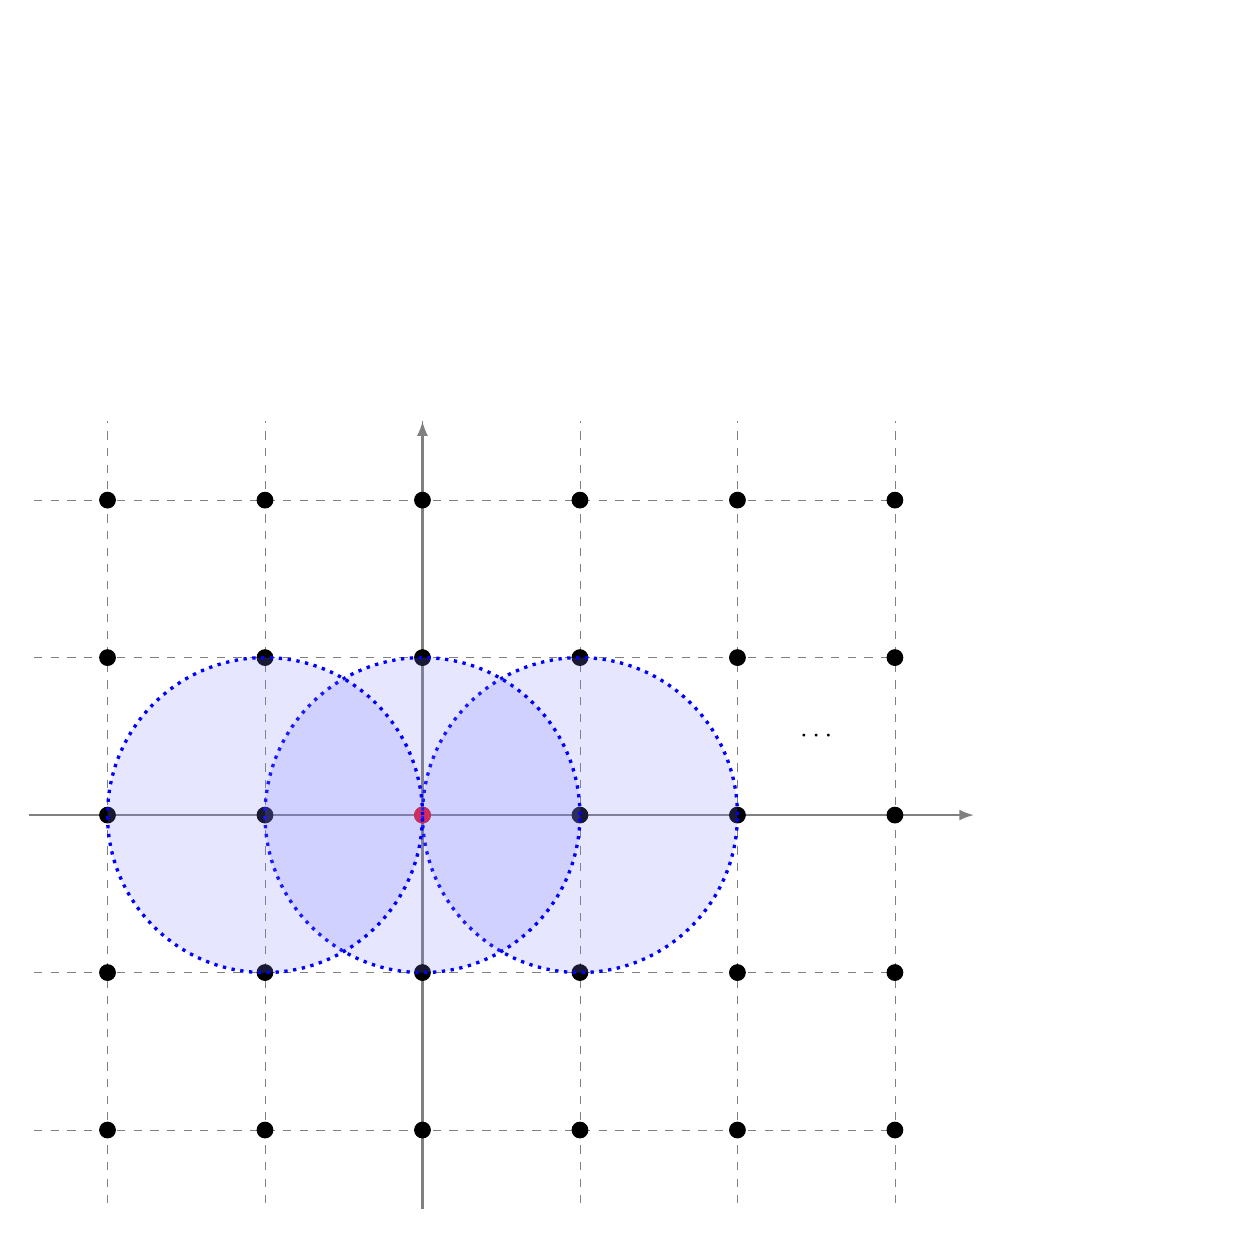
\begin{tikzpicture}
    \draw [thick, gray,-latex] (-5, 0) -- (7, 0);% Draw x axis
    \draw [thick, gray,-latex] (0, -5) -- (0, 5);% Draw y axis

    \clip (-5,-5) rectangle (10cm,10cm); % Clips the picture...
    %\pgftransformcm{1}{0.6}{0.7}{1}{\pgfpoint{0cm}{0cm}}
          % This is actually the transformation matrix entries that
          % gives the slanted unit vectors. 
    \draw[style=help lines,dashed] (-14,-14) grid[step=2cm] (6,5);
          % Draws a grid in the new coordinates.
          %\filldraw[fill=gray, fill opacity=0.3, draw=black] (0,0) rectangle (2,2);
              % Puts the shaded rectangle
    \foreach \x in {--3,-2,-1,0,1,2}{% Two indices running over each
      \foreach \y in {-2,-1, ..., 2}{% node on the grid we have drawn 
        \node[draw,circle,inner sep=2pt,fill] at (2*\x,2*\y) {};
            % Places a dot at those points
      }
    }
        \node[draw,red, circle,inner sep=2pt,fill] at (0, 0) {};

\filldraw[dotted, fill=blue!50, draw=blue, very thick, fill opacity=0.2] (2,0) circle (2cm);
\filldraw[dotted, fill=blue!50, draw=blue, very thick, fill opacity=0.2] (0,0) circle (2cm);
\filldraw[dotted, fill=blue!50, draw=blue, very thick, fill opacity=0.2] (-2,0) circle (2cm);
\node at (5, 1) {$\cdots$};
\end{tikzpicture}
}
\end{figure}

Continuing this way, every point with rational coordinates can be
covered by some open disc of radius 1:

\begin{figure}
\centering
\resizebox{\columnwidth}{!}{%
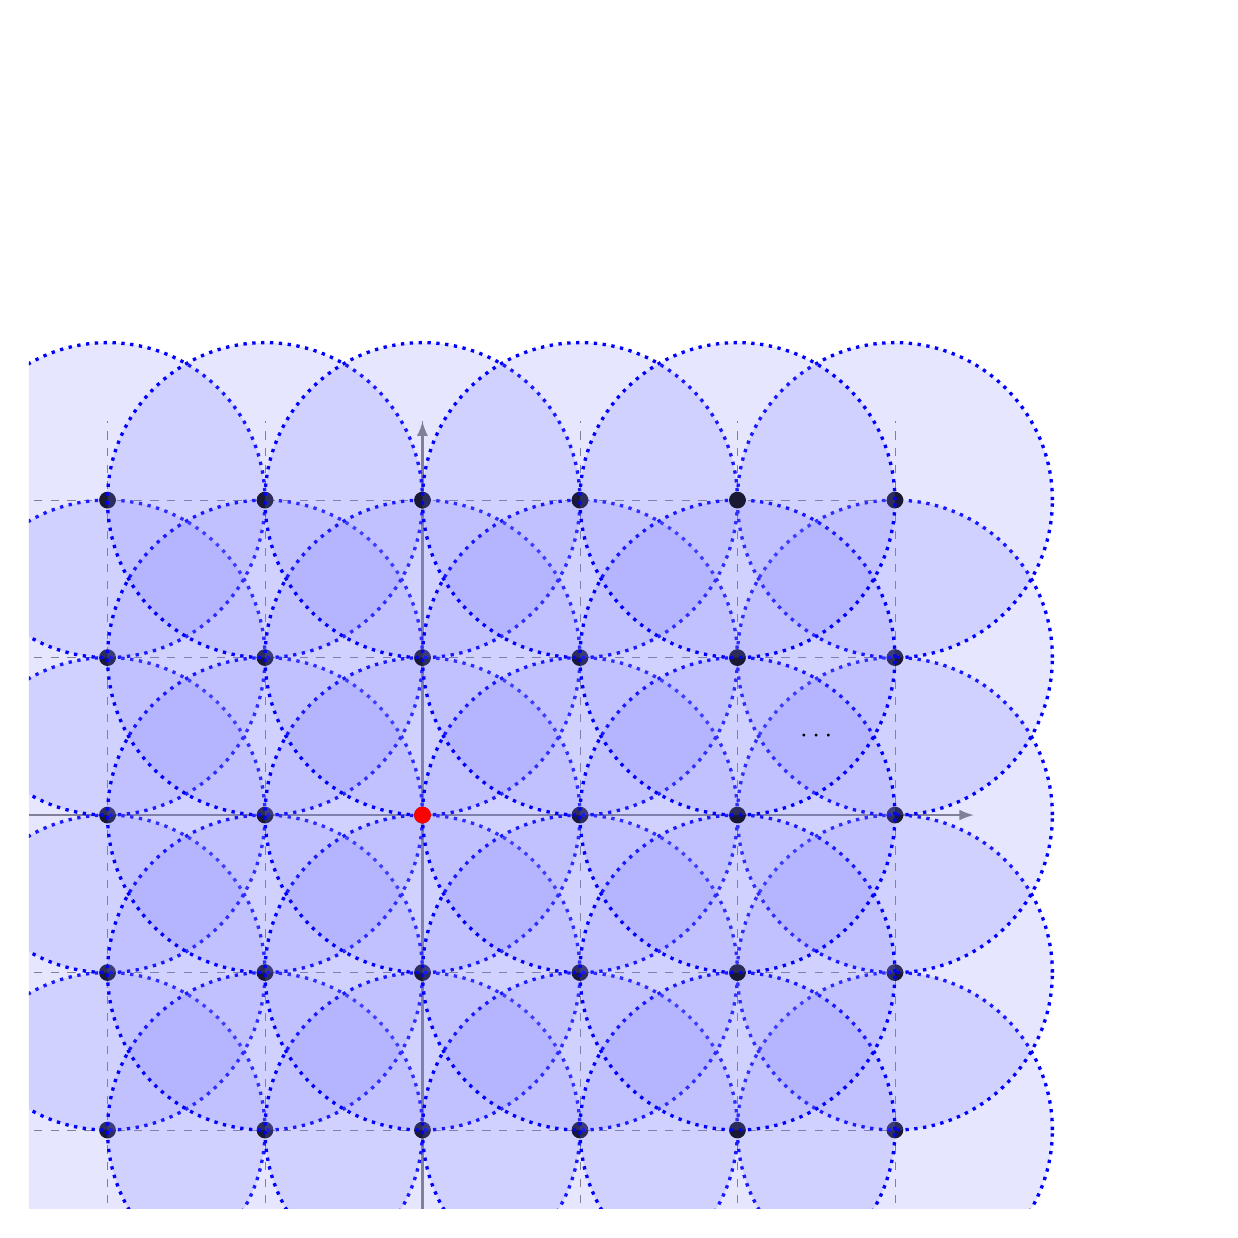
\begin{tikzpicture}
    \draw [thick, gray,-latex] (-5, 0) -- (7, 0);% Draw x axis
    \draw [thick, gray,-latex] (0, -5) -- (0, 5);% Draw y axis

    \clip (-5,-5) rectangle (10cm,10cm); % Clips the picture...
    %\pgftransformcm{1}{0.6}{0.7}{1}{\pgfpoint{0cm}{0cm}}
          % This is actually the transformation matrix entries that
          % gives the slanted unit vectors. 
    \draw[style=help lines,dashed] (-14,-14) grid[step=2cm] (6,5);
          % Draws a grid in the new coordinates.
          %\filldraw[fill=gray, fill opacity=0.3, draw=black] (0,0) rectangle (2,2);
              % Puts the shaded rectangle
    \foreach \x in {--3,-2,-1,0,1,2}{% Two indices running over each
      \foreach \y in {-2,-1, ..., 2}{% node on the grid we have drawn 
        \node[draw,circle,inner sep=2pt,fill] at (2*\x,2*\y) {};
\filldraw[dotted, fill=blue!50, draw=blue, very thick, fill opacity=0.2] (2*\x,2*\y) circle (2cm);

            % Places a dot at those points
      }
    }
        \node[draw,red, circle,inner sep=2pt,fill] at (0, 0) {};


\node at (5, 1) {$\cdots$};
\end{tikzpicture}
}
\end{figure}

\end{example}

\begin{remark}

Note that this doesn't work for arbitrary \(d\), since the distance
between the horizontal lines grows with \(d\). It's not hard to work out
the exact list where everything \emph{is} covered:

\end{remark}

\begin{theorem}[?]

\(K\) is norm-Euclidean if and only if
\(d\in \left\{{-1,-2,-3,-7,-11}\right\}\).

\end{theorem}

\begin{corollary}[?]

For these \(d\), \({\mathbb{Z}}_K\) is a PID and thus a UFD.

\end{corollary}

\begin{remark}

So we've classified all norm-Euclidean imaginary quadratic fields. What
about removing the word ``norm''? We restricted to
\({\left\lvert {N({\,\cdot\,})} \right\rvert}\) because there was a
particularly nice geometric interpretation, whereas being Euclidean
involves a mysterious \(\varphi\). Remarkably, it can be done, and it's
the same list!

\end{remark}

\begin{theorem}[Motzkin]

For \(K\) an imaginary quadratic field, \(K\) is Euclidean if and only
if \(d\in \left\{{-1,-2,-3,-7,-11}\right\}\).

\end{theorem}

\begin{remark}

If \({\mathbb{Z}}_K\) were never a PID in these cases, we could
immediately conclude it wasn't Euclidean either. But there are values of
\(d\) not on this list for which \({\mathbb{Z}}_K\) is a PID,
e.g.~\(d=-19\). Since \(-19 \equiv 1 \pmod 4\), one can write
\({\mathbb{Z}}_K = {\mathbb{Z}}\left[ {1 + \sqrt{-19} \over 2}\right]\),
and by Motzkin's theorem this is a PID which is not a Euclidean domain.

\end{remark}

We'll prove this theorem! First we need a few lemmas.

\begin{lemma}[?]

Let \(K\) be an imaginary quadratic field, then
\(U({\mathbb{Z}}_K) = \left\{{\pm 1 }\right\}\) except if \(d=-1, -3\).

\end{lemma}

\begin{proof}[of lemma (Important!)]

We know that the units \(u\) satisfy
\({\left\lvert {N(u)} \right\rvert} = 1\), and for imaginary quadratic
fields norms are non-negative, so we know \(N(u) = 1\). What are the
solutions this equation? Suppose \(d=2,3 \pmod 4\), then we can write
\(\alpha = a + b \sqrt{d}\) with \(a,b\in {\mathbb{Z}}\) and
\(1 = N \alpha = a^2 - db^2 = a^2 + {\left\lvert {d} \right\rvert}b^2\).
If \({\left\lvert {d} \right\rvert}= 1\) then this will have four
solutions: \((a, b) = (\pm 1, 0), (0, \pm 1)\). Otherwise if
\({\left\lvert {d} \right\rvert}> 1\) then \(b=0\) and
\(a^2=1 \implies a = \pm 1\) and thus \(\alpha = \pm 1\). So in this
case, the only units are \(\pm 1\), unless
\({\left\lvert {d} \right\rvert} = 1\). But the only negative squarefree
integer of absolute value 1 is \(-1\).

Suppose \(d \equiv 1 \pmod 4\). In this case, we need
\begin{align*}
1 = {a^2 + {\left\lvert {d} \right\rvert} b^2 \over 4} \implies a^2 + {\left\lvert {d} \right\rvert}b^2 = 4  
.\end{align*}
Note that \(d<0\) is \(1\pmod 4\), so it's possible that \(d=-3\) -- but
this was one of the exceptions in the theorem, so assume otherwise. Thus
\({\left\lvert {d} \right\rvert}\geq 7\), which forces
\(b=0 \implies a^2 = 4 \implies a = \pm 2\). Then \(\alpha= \pm 1\).

\end{proof}

\begin{remark}

For the excluded cases, the units can be explicitly computed. When
\(d=-1\), \(U({\mathbb{Z}}[i]) =\left\{{\pm 1, \pm i}\right\}\),
yielding 4 units. When \(d=-3\),
\begin{align*}
U\qty{{\mathbb{Z}}\left[ {1 + \sqrt{-3} \over 2 } \right]} = \left\{{\pm 1, {\pm 1 \pm \sqrt{-3} \over 2}}\right\}
,\end{align*}
yielding 6 units. Note that in the first case, these are exactly the 4th
roots of unity, and in the second case these are the sixth roots. This
is a general phenomenon that will appear again!

\end{remark}

\begin{lemma}[?]

Let \(K\) be any quadratic field and \(\alpha\in {\mathbb{Z}}_K\). Then
\(\# {\mathbb{Z}}_k / \left\langle{ \alpha }\right\rangle = {\left\lvert {N( \alpha )} \right\rvert}\).

\end{lemma}

\hypertarget{proof-of-motzkins-theorem}{%
\subsection{Proof of Motzkin's
Theorem}\label{proof-of-motzkins-theorem}}

\begin{proof}[of Motzkin's Theorem]

We want to show that being Euclidean implies \(d=-1,-2,-3,-7,-11\).
Suppose \({\mathbb{Z}}_K\) is Euclidean with respect to \(\varphi\).
Choose \(\beta\in {\mathbb{Z}}_K\) nonzero and not a unit with
\(\varphi(\beta)\) minimal among all such \(\beta\).

\begin{claim}

\begin{align*}
\# {\mathbb{Z}}_K / \left\langle{ \beta }\right\rangle \leq 3 
.\end{align*}

\end{claim}

\begin{proof}[of claim]

For any \(\alpha\in {\mathbb{Z}}_K\) and consider it in the quotient.
Since \({\mathbb{Z}}_K\) is Euclidean, we can write
\(\alpha = \beta + \gamma+ \rho\) where either \(\rho=0\) or
\(\varphi(\rho ) < \varphi (\beta )\). How can the second possibility
occur? \(\beta\) was chosen to have a minimal \(\varphi\) value, so the
only smaller elements are units. So \(\rho = 0\) or \(\rho\) is a unit.
Reducing \(\pmod\beta\), we obtain \(\alpha= \rho \pmod\beta\), and
hence
\(\# {\mathbb{Z}}_K / \left\langle{ \beta }\right\rangle \leq 1 + \# U({\mathbb{Z}}_K)\)
where the 1 comes from the zero element and everything else in the
quotient has a representative that is a unit. This is bounded above by
\(3\) when \(d\neq -1, -3\), which is one of the exclusions in the
theorem.

\end{proof}

Now we have \(N( \beta) \leq 3\) and this can be solved -- if \(d\) is
large, these solutions are widely distributed. If \(d = 2, 3 \pmod 4\)
then \(\beta= a + b \sqrt{d}\) with \(a, b \in ZZ\) and
\(a^2 + {\left\lvert {d} \right\rvert}b^2 \leq 3\). We can assume
\({\left\lvert {d} \right\rvert}> 3\), since \(d=-1, -2\) are excluded.
Then \(b=0\) is forced, and \(a = 0, \pm 1\). But why can't
\(\beta=0, \pm 1\)? It was chosen to be minimal among \emph{nonzero
nonunits}. \(\contradiction\)

If \(d \equiv 1 \pmod 4\), then \(\beta= {a + b \sqrt{d} \over 2}\)
where \(a,b\in {\mathbb{Z}},\, a\equiv b \pmod 2\). Then
\begin{align*}
{a^2 + {\left\lvert {d} \right\rvert}b^2 \over 4} \leq 3 \implies a^2 + {\left\lvert {d} \right\rvert}b^2 \leq 12  
.\end{align*}
Now considering that
\(-d\equiv 1 \pmod 4 \implies -d \in \left\{{ -3, -7, -11, \cdots}\right\}\),
the first three of which are on our list of exclusions. So we can assume
\({\left\lvert {d} \right\rvert}\geq 15\), which forces \(b=0\), \(a\)
must be even, and \(a^2 \leq 12\). So
\(a=0, \pm 2 \implies \beta= 0, \pm 1\). \(\contradiction\)

\end{proof}

\begin{remark}

What's the story for real quadratic fields? We understand norm-Euclidean
ones, although the proofs aren't nearly as simple. Things worked out
nicely here because we had circles in the plane; in the real case these
end up being complicated hyperbolas. One can prove that if \(d > 73\)
then \(K \coloneqq{\mathbb{Q}}(\sqrt d)\) is not norm-Euclidean. What
are the Euclidean real quadratic fields? The situation is much
different, and there are two open conjectures.

\end{remark}

\begin{conjecture}

For real quadratic fields \(K\), \({\mathbb{Z}}_K\) is a PID for
infinitely many \(d> 0\). We don't even know about to prove there are
just infinitely many \emph{number} fields satisfying this condition! We
believe this is true since it happens a positive proportion of the time
experimentally.

\end{conjecture}

\begin{conjecture}

If \({\mathbb{Z}}_K\) is a PID, then \({\mathbb{Z}}_K\) is Euclidean
with respect to some norm function. This is a consequence of a certain
generalization of the RH. This is not true for imaginary quadratic
fields. Why is it different here? The unit group plays a large role, and
is infinite here. The real conjecture is that for \(K\) any number
field, if \({\mathbb{Z}}_K\) is a PID with infinitely many units then
\({\mathbb{Z}}_K\) is Euclidean.

\end{conjecture}

\begin{remark}

There has been some progress, a result along the lines of there being at
most two exceptions, but we don't know if those exceptions exist.

\end{remark}

\addsec{ToDos}
\listoftodos[List of Todos]
\cleardoublepage

% Hook into amsthm environments to list them.
\addsec{Definitions}
\renewcommand{\listtheoremname}{}
\listoftheorems[ignoreall,show={definition}, numwidth=3.5em]
\cleardoublepage

\addsec{Theorems}
\renewcommand{\listtheoremname}{}
\listoftheorems[ignoreall,show={theorem,proposition}, numwidth=3.5em]
\cleardoublepage

\addsec{Exercises}
\renewcommand{\listtheoremname}{}
\listoftheorems[ignoreall,show={exercise}, numwidth=3.5em]
\cleardoublepage

\addsec{Figures}
\listoffigures
\cleardoublepage


\printbibliography[title=Bibliography]


\end{document}
